% Tento soubor nahraďte vlastním souborem s obsahem práce.
%=========================================================================
% Autoři: Michal Bidlo, Bohuslav Křena, Jaroslav Dytrych, Petr Veigend a Adam Herout 2019

% Pro kompilaci po částech (viz projekt.tex), nutno odkomentovat a upravit
%\documentclass[../projekt.tex]{subfiles}
%\begin{document}

\chapter{Úvod}
\label{introduction}

Záměrem této práce je ukázat možné uplatnění formálních modelů v interdisciplinární oblasti informatiky a vizuálního umění. Konkrétní aplikaci těchto modelů nacházím ve spojení barevné palety, jednoduchých tvarů, a systému dlaždic -- mřížky. V rámci teoretické části je navržena a popsána sada dvou-dimenzionálních automatů, které představují formální základ pro aplikaci schopnou vytvořit nové vizuální dílo syntézou tří výše uvedených vstupů. 

Praktickou část představuje implementace programu, který rozpoznává mřížku definovanou uživatelem a obohacuje ji o barvy, které extrahuje z jiného obrazu. Tento proces můžeme chápat jako spolupráci uživatele, který poskytuje mřížku a barevný obraz, a programu, syntetizujícího obojí do nového díla. Výsledná aplikace vytvoří několik verzí barevných mozaiek, sestávajících z obarvených dlaždic, které na konci sloučí do nového díla -- videa. 

Hlavní inspirace pro tuto práci jsem nalezl zejména v sériovém umění maďarského umělce Victora Vasarelyho, který v tomto stylu tvořil v 60. letech 20. století v rámci směru op-art. Sériové umění pro Vasarelyho znamenalo práci s abecedou tvarů a barev, které různě aranžoval a jejichž kombinací tvořil několik variant jednoho obrazu. 

\begin{displayquote}
\emph{,,Plastická abeceda se stane výchozím bodem kolektivního umění. Hra s kombinacemi a permutacemi umožní vznik řady návrhů díky kombinaci forem a jemných rozdílů v rozmezích definovaných autorem.''}\\
    \bigskip
    \hfill \,--\,  Victor Vasarely \cite{museum}
\end{displayquote}

Návrh aplikace navazuje na Vasarelyho hru s permutacemi, která je uvedena v citaci výše. Uživatel může aplikaci několika způsoby omezovat, dostává prostor experimentovat s různými vstupy, a konečně může pozorovat, jak se jeho výběr barev a tvarů projevuje v~kombinaci se vstupní mřížkou na snímcích, vytvořených aplikací. 

Jiný zdroj inspirace pochází z bakalářských prací Mária Gaža a Martiny Zlevorové, kteří se věnovali podobnému tématu, ale na rozdíl od této práce se zaměřili na kompozici textu. Čerpal jsem zejména z jejich využití celulárních automatů pro řazení a rozprostření písmen po obrazu. Celulární automat byl v této práci navržen tak, aby místo textu dokázal modifikovat obsah a pořadí dlaždic v mřížce.

V \hyperref[current]{následující kapitole} se věnuji zejména existujícím formálním modelům, které bylo třeba nastudovat pro rozpoznání a transformaci vstupní mřížky. Čtenář, který není s dvou-dimenzionálními automaty obeznámen, se v této kapitole dozví klíčové pojmy a definice, potřebné pro pochopení návrhu nových modelů. Okrajově se zde věnuji použití formálních modelů v umění a zasazuji práci do kontextu interdisciplinárního prostoru mezi uměním a~informatikou, ve kterém vznikala. 

\hyperref[newAutomata]{Třetí kapitola} obsahuje návrhy nových automatů, které působí na vstupní mřížce. Navržené modely plní roli rozpoznání, modifikace, a transformace nad vstupní mřížkou a~reprezentují formální návrh klíčových řídících prvků implementované aplikace. Popsána je zejména činnost samotných modelů, ale současně i jejich role v kontextu celé aplikace. Kromě modelů jsou v této kapitole popsány parametry vstupní mřížky a dlaždic, které je automat schopen správně rozpoznat.

Následuje \hyperref[impl]{implementační kapitola}, ve které se nachází popis struktury aplikace, návod na její spuštění, a výčet technologií použitých při implementaci. Struktura programu je popsána nejprve z vysokoúrovňového procedurálního pohledu a následně z bližšího pohledu na jednotlivé moduly aplikace. Je zde uvedeno, jaké funkce moduly plní a jakým způsobem implementují návrh popsaný v předchozí kapitole. 

Testování aplikace a ukázky výstupů se nachází v \hyperref[testing]{páté kapitole}. Na jednotlivých ukázkách jsou zde znázorněny výstupy, které byly za pomocí určitých vstupů získány. Zároveň je zde zahrnuta úvaha nad kvalitou výsledků včetně případů, kdy byly výsledky aplikace neuspokojivé. Čtenář, který má zájem shlédnout především výstupy aplikace, může diagramy obsažené v této kapitole studovat jako první.

V \hyperref[conclusion]{poslední kapitole} je práce shrnuta a zhodnocena z hlediska splnění zadání. Jsou zde zmíněny přednosti a nedostatky práce společně s vizí budoucího vývoje.

\chapter{Dvou-dimenzionální automaty využité pro zpracování obrazu}
\label{current}

Automaty představují v kontextu formálních modelů jeden z možných přístupů ke konceptualizaci formálních jazyků. Mezi ostatní přístupy můžeme řadit například gramatiky a výrazy. Automaty jsou pro nás významné tím, že nám umožňují na rozdíl od gramatik a výrazů nahlížet na formální jazykové modely jiným způsobem, jelikož jazyky negenerují, ale přijímají \cite{MedunaAlexander2012Aalt}. Pro zaměření této práce jsou klíčové modely, které jsou schopny pracovat s dvou-dimenzionálním obrazem, který chceme rozpoznat, abstrahovat, a transformovat. Jako teoretický základ byly vybrány dva modely, které umí přijmout jazyk obrazů. Konkrétně se jedná o čtyřcestný automat, který sekvenčně prochází obraz, a celulární automat, který obraz celkově transformuje v jednom kroku \cite{RozenbergGrzegorz1997HoFL}. 

V následujících sekcích je objasněn princip těchto modelů, společně s jejich formálními definicemi a příklady jejich využití. 

\section{Základní definice spojené s automaty}

Níže je uvedeno několik základních definic a pojmů spojených s teorií formálních modelů, které je potřeba znát pro celistvé pochopení automatů definovaných v následujících sekcích.

\subsection*{Dílčí pojmy}
\begin{description}
    \item[Abeceda] je konečná neprázdná množina znaků, které nazýváme symboly. Značíme ji písmenem $\Sigma$ \cite{MedunaAlexander2012Aalt}.  Příkladem jednoduché abecedy je množina číslic binární soustavy, kterou formálně zapíšeme jako: $\Sigma = \{0, 1\}$.
    
    \item[Slovo] je neformálně definováno jako řetězec symbolů. Řetězec, který získáme spojením znaků z abecedy $\Sigma$ nazýváme slovo nad $\Sigma$. Množina všech takových slov, včetně prázdného řetězce $\epsilon$, se značí $\Sigma^{*}$ \cite{MedunaAlexander2012Aalt}.
    
    \item[Jazyk] $L$ je podmnožinou $\Sigma^{*}$, formálně zapsáno jako: $L \subseteq \Sigma^{*}$ \cite{MedunaAlexander2012Aalt}. Příklad jazyku abecedy $\Sigma = \{0, 1\}$ je například jazyk slov, které obsahují pouze 2 znaky: $L = \{01, 10, 00, 11\}$.
    
    \item[Obraz] můžeme chápat jako dvou-dimenzionální řetězec, jenž je formálně definován jako dvou-dimenzionální obdélníkové pole znaků nad abecedou $\Sigma$. Při přechodu do dvou dimenzí nastává změna v notaci množiny všech obrazů nad $\Sigma$, kterou zapisujeme jako $\Sigma^{**}$. Podmnožinu $\Sigma^{**}$ nazýváme jazykem obrazů. Obraz $p \in \Sigma^{**}$, kde $l_{1}(p)$ je počet řádků obrazu a  $l_{2}(p)$ je počet sloupců, má rozměry definované jako $(l_{1}(p), l_{2}(p))$ \cite{RozenbergGrzegorz1997HoFL}.
\end{description}

\subsection*{Deterministický konečný automat}

Jako příklad pro snažší pochopení vícedimenzionálních automatů je níže uvedena definice jednodimenzionálního deterministického konečného automatu, též často nazývaného zkratkou \emph{DFA} (z ang. Discrete Finite Automaton).

Deterministický automat se vyznačuje tím, že jeho tranzitivní funkce $\delta$ pro nějaký stav a symbol na vstupu vrátí \emph{právě jeden} stav na výstupu \cite{HopcroftJohnE.2007Itat}. Všechny automaty, které jsou v~této práci navrženy, disponují touto vlastností -- jsou deterministické.


\begin{definition}
Deterministický konečný automat (DFA) je pětice $(Q, \Sigma, \delta, q_{0}, F)$, blíže definována níže \cite{HopcroftJohnE.2007Itat}:
\begin{itemize}
    \item $Q$ je \emph{konečná} množina stavů,
    \item $\Sigma$ je \emph{konečná} množina vstupních symbolů,
    \item $\delta$ je tranzitivní funkce, přičemž pro stav $q \in Q$ a vstupní symbol $a\in \Sigma$ platí: \linebreak $\delta(q, a) = p$ a zároveň $p \in Q$,
    \item $q_{0}$ Je počáteční stav z množiny $Q$,
    \item $F$ je množina konečných stavů, pro které platí: $F \subset Q$.
\end{itemize}
\end{definition}

\subsection*{Diagram přechodů}
Automaty můžeme specifikovat několika způsoby, například definicí tranzitivní funkce, nebo pomocí tabulky přechodů. V této práci jsem se rozhodl automaty specifikovat pomocí diagramu přechodů, jelikož se jednoduše přepisuje do procedurálního kódu a vede k přímočaré implementaci. Níže je uvedena definice diagramu přechodů společně s příklady notací jeho dílčích složek, která je v této práci využita. 

\begin{definition}
Diagram přechodů je pro deterministický konečný automat definován následovně \cite{HopcroftJohnE.2007Itat}:
\begin{itemize}
    \item Pro každý stav z množiny $Q$ existuje uzel. 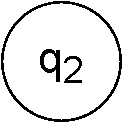
\includegraphics[scale=0.3]{obrazky-figures/Stav.pdf}
    \item Pro každý stav $q \in Q$, vstupní symbol $a\in \Sigma$ a tranzitivní funkci $\delta(q, a) = p$, $p \in Q$, existuje v diagramu přechod označený jako $a$. 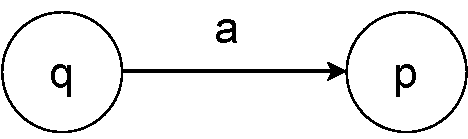
\includegraphics[scale=0.3]{obrazky-figures/Prechod.pdf}
    \item Počáteční stav $q_{0}$ je označen přechodem, který nemá počátek v žádném uzlu a je označen slovem $Start$. 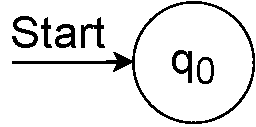
\includegraphics[scale=0.3]{obrazky-figures/StartStav.pdf}
    \item Koncový stav, který náleží množině $F$, je znázorněn jako uzel sestávající z dvou koncentrických kruhů.  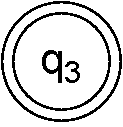
\includegraphics[scale=0.3]{obrazky-figures/FinalStav.pdf}
\end{itemize}
\end{definition}


\section{Čtyřcestné (skákající) automaty}

Čtyřcestné automaty využil ke zpracování obrazu Ing. Dominik Švač ve své bakalářské \cite{BakalarkaSvac} a~diplomové \cite{DiplomkaSvac} práci. Schopnost automatů přijmout vstupní obraz aplikoval pro rozpoznání dopravních značek a číslic. Návrhy Ing. Švače byly primární inspirací při tvorbě čtyřcestných automatů pro rozpoznání mřížky. V této sekci uvedu teoretické základy pro pochopení principu činnosti čtyřcestných automatů a zároveň seznámím čtenáře s konceptem skoků a jejich využitím v této práci.

\subsection*{Čtyřcestný konečný automat}
Čtyřcestný konečný automat, též v angličtině nazývaný zkratkou \emph{4FA}, je formálně definován jako rozšíření dvoucestného automatu, který čte jednorozměrné řetězce \cite{RozenbergGrzegorz1997HoFL}. 

Neformálně můžeme čtyřcestný automat chápat, když se zaměříme na aspekty, ve~kterých se liší od jednoduchého deterministického konečného automatu. Čtyři směry (nahoru, dolů, doleva, doprava) značí pohyb čtecí hlavice na vstupním dvojrozměrném řetězci -- obrazu. Jednoduchý automat (DFA) se vždy po přečtení znaku na jednorozměrné pásce posunul na další znak; čtyřcestný automat se může na pásce dvojrozměrné pohybovat ve~směrech figurky věže na šachovnici. Rozšíření automatu o další směry pohybu má dopad na~jeho tranzitivní funkci $\delta$.
Pro daný stav automatu a znak na vstupní pásce funkce $\delta$ vrátí nejen další stav, ale zároveň pohne s čtecí hlavicí v jednom ze čtyř směrů. Množina koncových stavů je u čtyřcestného automatu nahrazena dvěma stavy: přijímacím a o
zamítajícím stavem. Na základě toho, ve kterém stavu automat skončil, víme, zda byl obraz rozpoznán \cite{RozenbergGrzegorz1997HoFL}.

Tyto vlastnosti umožňují automatu vracet se k již navštíveným znakům na vstupní pásce, nebo určité znaky přeskakovat a zároveň zachovat kontinuální procházení (na rozdíl od konceptu skoků, který bude zmíněn v dalších sekcích, a představuje diskontinuální výpočet) \cite{MedunaFormalLang}. 

Vstupní obraz je ohraničen znaky, které představují ,,bod návratu'' automatu, pokud čtecí hlavice přečte takový znak, vrátí se zpět na předchozí přečtený. V této práci jsou hranice obrazu reprezentovány znakem $\#$.

Čtyřcestný automat definují D. Giammarresi a A. Restivo následovně:

\begin{definition}
Čtyřcestný konečný automat (4FA) je sedmice $(\Sigma, Q, \Delta, q_{0}, q_{a}, q_{r}, \delta)$, s~následujícím významem elementů \cite{RozenbergGrzegorz1997HoFL}:
\begin{itemize}
    \item $\Sigma$ je vstupní abeceda,
    \item $Q$ je \emph{konečná} množina stavů,
    \item $\Delta = \{R, L, U, D\}$ je množina povolených směrů,
    \item $q_{0}$ Je počáteční stav z množiny $Q$,
    \item $q_{a}$ Je přijímací stav z množiny $Q$,
    \item $q_{r}$ Je zamítající stav z množiny $Q$,
    \item $\delta$ je tranzitivní funkce, která je definována jako: $Q \setminus \{q_{a}, q_{r}\} \times \Sigma \longrightarrow 2^{Q \times \Delta}$.
\end{itemize}
\end{definition}

Následuje příklad pro ilustraci činnosti čtyřcestného automatu pomocí diagramu přechodů.

\begin{example}
Nechť je $\Sigma = \{0, 1\}$ abecedou a $L \subseteq \Sigma^{**}$ jazykem obrazů, jejichž první sloupec je roven sloupci poslednímu. Cílem je navrhnout automat, který bude přijímat právě jazyk $L$ \cite{RozenbergGrzegorz1997HoFL}.
\label{4FApriklad}
\end{example}

Řešení příkladu \ref{4FApriklad} je znázorněno na obrázku \ref{fig:reseni4FAprikladu} níže. K návrhu automatu pomohla jiná formulace původního problému. První sloupec je roven poslednímu právě tehdy, když jsou si na každém řádku rovny první a poslední znaky. 

Automat čte obrázek řádek po řádku, střídavě zleva doprava a poté zprava doleva. Obraz přijímá, pokud se nacházíme ve stavu přijetí $q_a$. Na diagramu přechodů je explicitně znázorněn návrat z hranic obrazu zpět (znak $\#$). Diagram je symetrický, horní část znázorňuje případy, kdy právě čteme řádek, kde je v prvním a posledním sloupci znak $0$, spodní část reprezentuje případ, kdy je stejném místě znak $1$. Automat obraz přijme až v situaci, kdy jsou přečteny všechny řádky. Pro přehlednost je v tomto diagramu přechodů vynechán zamítající stav $q_r$. Automat v tomto řešení obraz zamítá, když skončí ve stavu, který není stavem $q_a$, a už se nemůže dále pohnout. 

\begin{figure}[H]
    \centering
    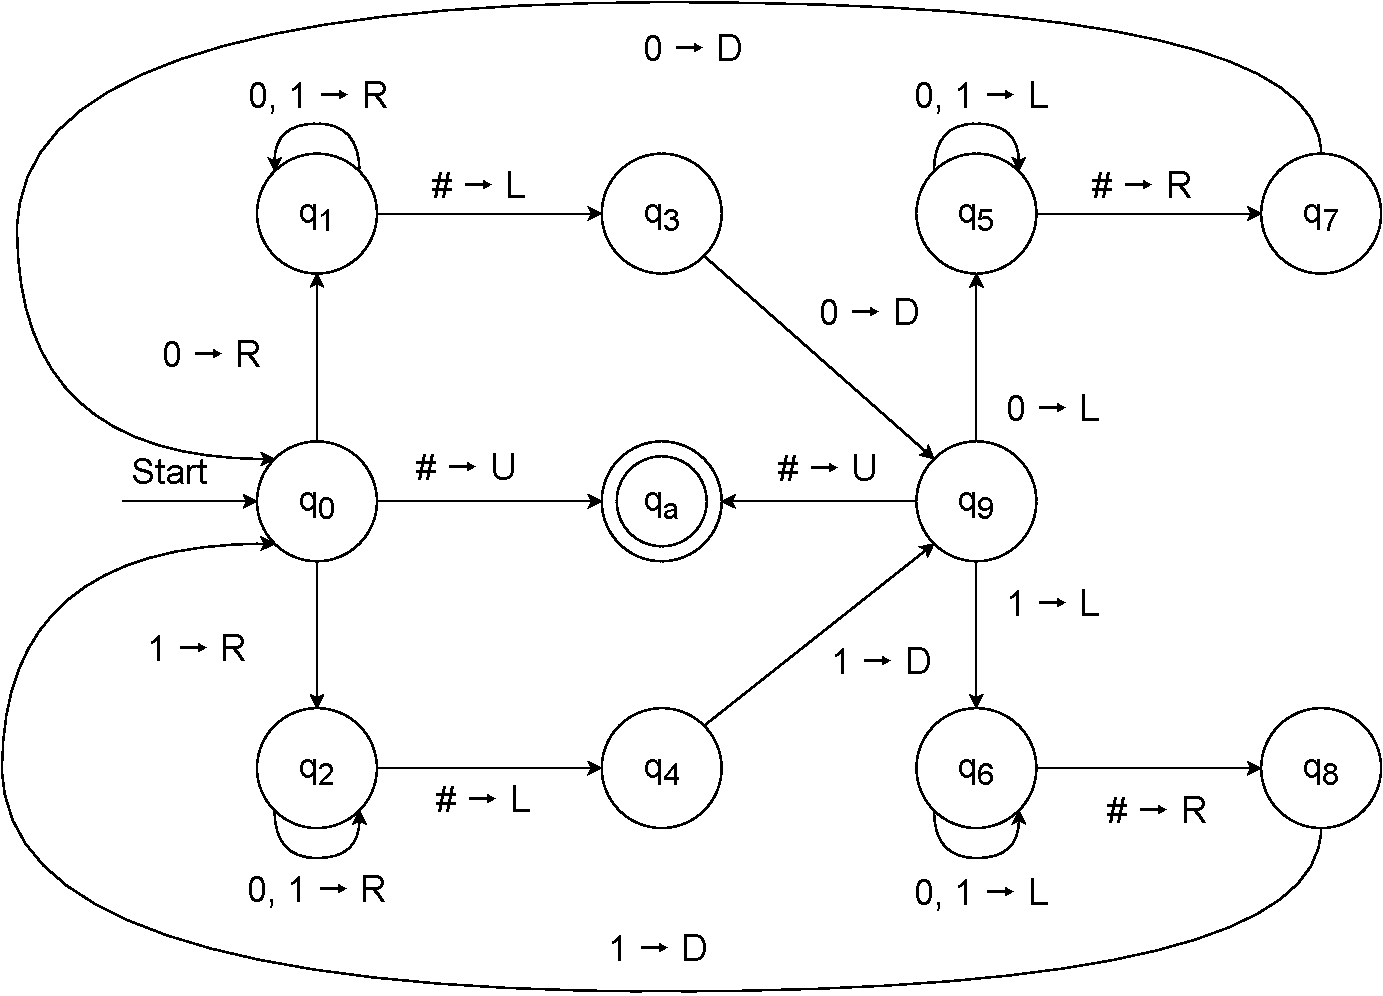
\includegraphics[width=\textwidth]{obrazky-figures/4FA_priklad.pdf}
    \caption{Řešení příkladu \ref{4FApriklad}}
    \label{fig:reseni4FAprikladu}
\end{figure}

\subsection*{Skoky v kontextu čtyřcestných automatů}
\label{skok}

Tato práce se zabývá skákajícími automaty jen velmi okrajově. Mají zde své místo kvůli tomu, že pomocí nich můžeme modelovat diskontinuální výpočet. V další kapitole se budeme zabývat rozpoznáním mřížky sestávající z dlaždic, vstupní obraz bude čten řádek po řádku, ale vždy zleva doprava. Skoky nám ušetří výpočetní čas tím, že se čtecí hlavice nebude muset vracet na nejlevější znak následujícího řádku, ale přesune se přímo na něj pomocí skoku. 

Z formálního hlediska jsou skoky rozšířením množiny pravidel (tranzitivní funkce) automatu \cite{DiplomkaSvac}. Níže je popsán druh skoku, který byl v této práci aplikován.

\begin{definition}
Skok na konkrétní místo vstupního obrazu je formálně zapsán následujícím způsobem: $xpaz \curvearrowright_{i, j} x'qz'$.
Přičemž $p, q \in Q, x, x', a, z, z' \in \Sigma^*$, $i$ značí řádek a $j$ značí sloupec, kam se přesune čítací hlavice.  \cite{DiplomkaSvac}. Na rozdíl od definice v práci Ing. Švače jsem se pro jednoduchost rozhodl vynechat koncept přečtených symbolů, uvažuji pouze množinu $\Sigma$.

Speciální případ tohoto skoku je skok na začátek dalšího řádku, který je v této práci využit a je zapsán jako: $xpaz \curvearrowright_{+1, 1} x'qz'$ \cite{DiplomkaSvac}.
\end{definition} 

\section{Celulární automaty}

Celulární automaty (zkratkou často \emph{CA}) využívají v porovnání s čtyřcestnými automaty jiný přístup k zpracování vstupního obrazu. Vstupní obraz celulární automaty konceptualizují jako (dvou-dimenzionální) pole buněk, které se v každém okamžiku nachází v právě jednom z $k$ stavů, přičemž platí, že $(k \geq 2)$. V této práci se budeme zabývat celulárními automaty s buňkami ve tvaru čtverce, ale obecně existují buňky různých tvarů \cite{CATheory}. 

Samotné zpracování vstupního obrazu u celulárního automatu neprobíhá sekvenčně, buňku po buňce, ale prostřednictvím totálního přechodu, ve kterém se v jednom časovém bodě změní všechny buňky současně \cite{RozenbergGrzegorz1997HoFL}. Celulární automat využívá diskrétní čas, buňky se v časových krocích mění, přičemž s každým krokem je čas inkrementován. Změna stavů buněk je definována lokální tranzitivní funkcí, která se synchronně v jednom kroku aplikuje na všechny buňky. Funkce mění stav buňky v závislosti na nějakém lokálním okolí, skládajícím se z ostatních buněk, které nazýváme sousedy. Výsledkem přiřazení stavů do celého pole buněk je \emph{konfigurace} v určitém čase. Celulární automat můžeme definovat jako trojici, kterou tvoří pole buněk, množina povolených stavů, a tranzitivní funkce \cite{CATheory}.

Dvou-dimenzionální celulární automaty v jednom kroku zpracovávají celý obraz. Jejich tranzitivní funkce pracují s dvěma elementárními druhy okolí, které se jmenují \emph{Moorovo} a~\emph{Von Neumannovo}. V případě okolí dvou-dimenzionálních CA mluvíme o poloměru $r$, který značí jeho velikost \cite{CATheory}. 

\begin{figure}[H]
    \centering
    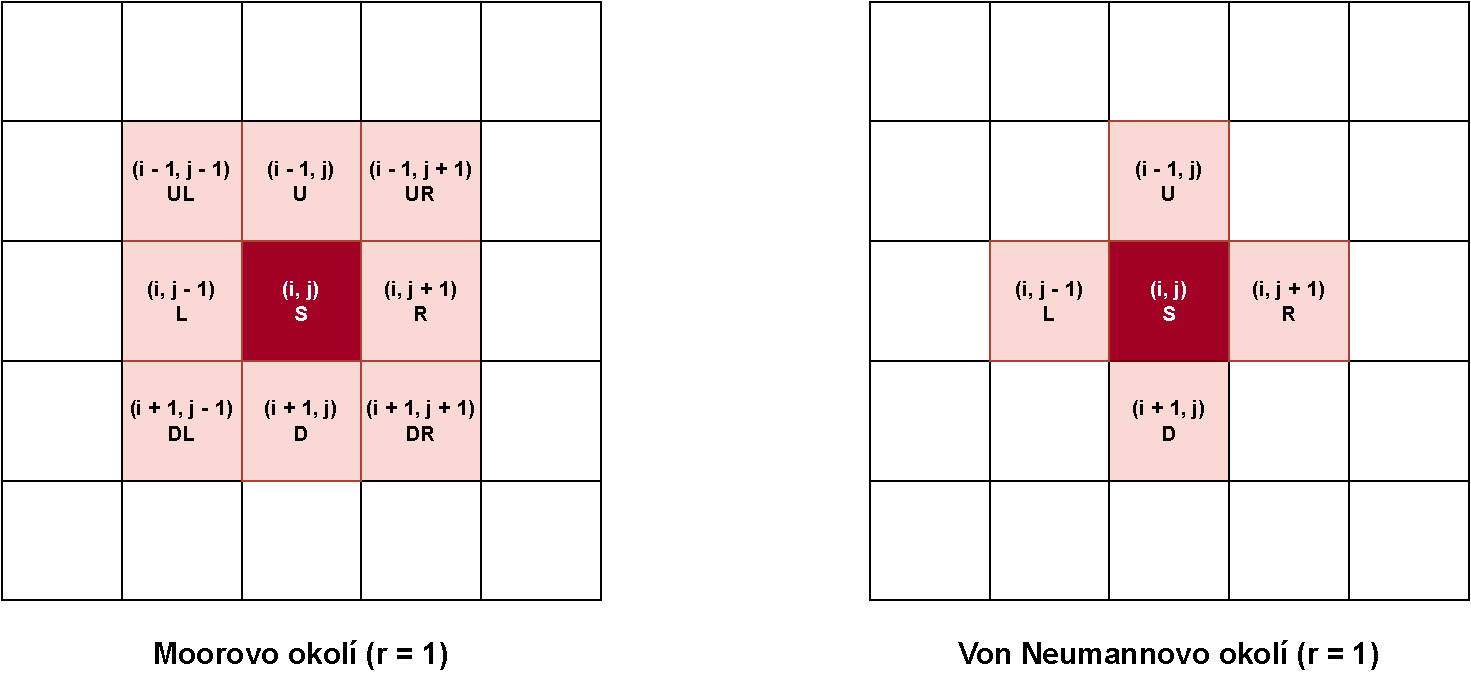
\includegraphics[width=\textwidth]{obrazky-figures/CAOkoli.pdf}
    \caption{Základní druhy okolí u 2D celulárních automatů}
    \label{fig:CAOkoli}
\end{figure}

\subsection*{Aplikace celulárních automatů v umění}
Umělecký potenciál můžeme u celulárních automatů najít v jejich vlastnosti generovat nečekané a komplexní vzory na základě jednoduchých pravidel. Šíři potenciálu těchto modelů ilustruje fakt, že mnoho různých uměleckých děl může vzniknout z jediného návrhu. Jako příklad můžeme využít celulární automat \emph{Game of Life} (zkráceně Life) Johna Conwaye, pomocí kterého můžeme pouhou změnou počátečních konfigurací a využitím rozdílných barevných palet vytvářet široké spektrum komplexních ornamentů a jedinečných obrazů, transformujících se v čase \cite{CAArt}. Na diagramu \ref{fig:caUmeni} jsou znázorněny dva obrazy, pro jejichž tvorbu byl využit automat Life.

\begin{figure}[H]
    \centering
    \includegraphics[width=0.4\textwidth]{obrazky-figures/lifeWOdeath.png}
    \hspace{0.1\textwidth}
    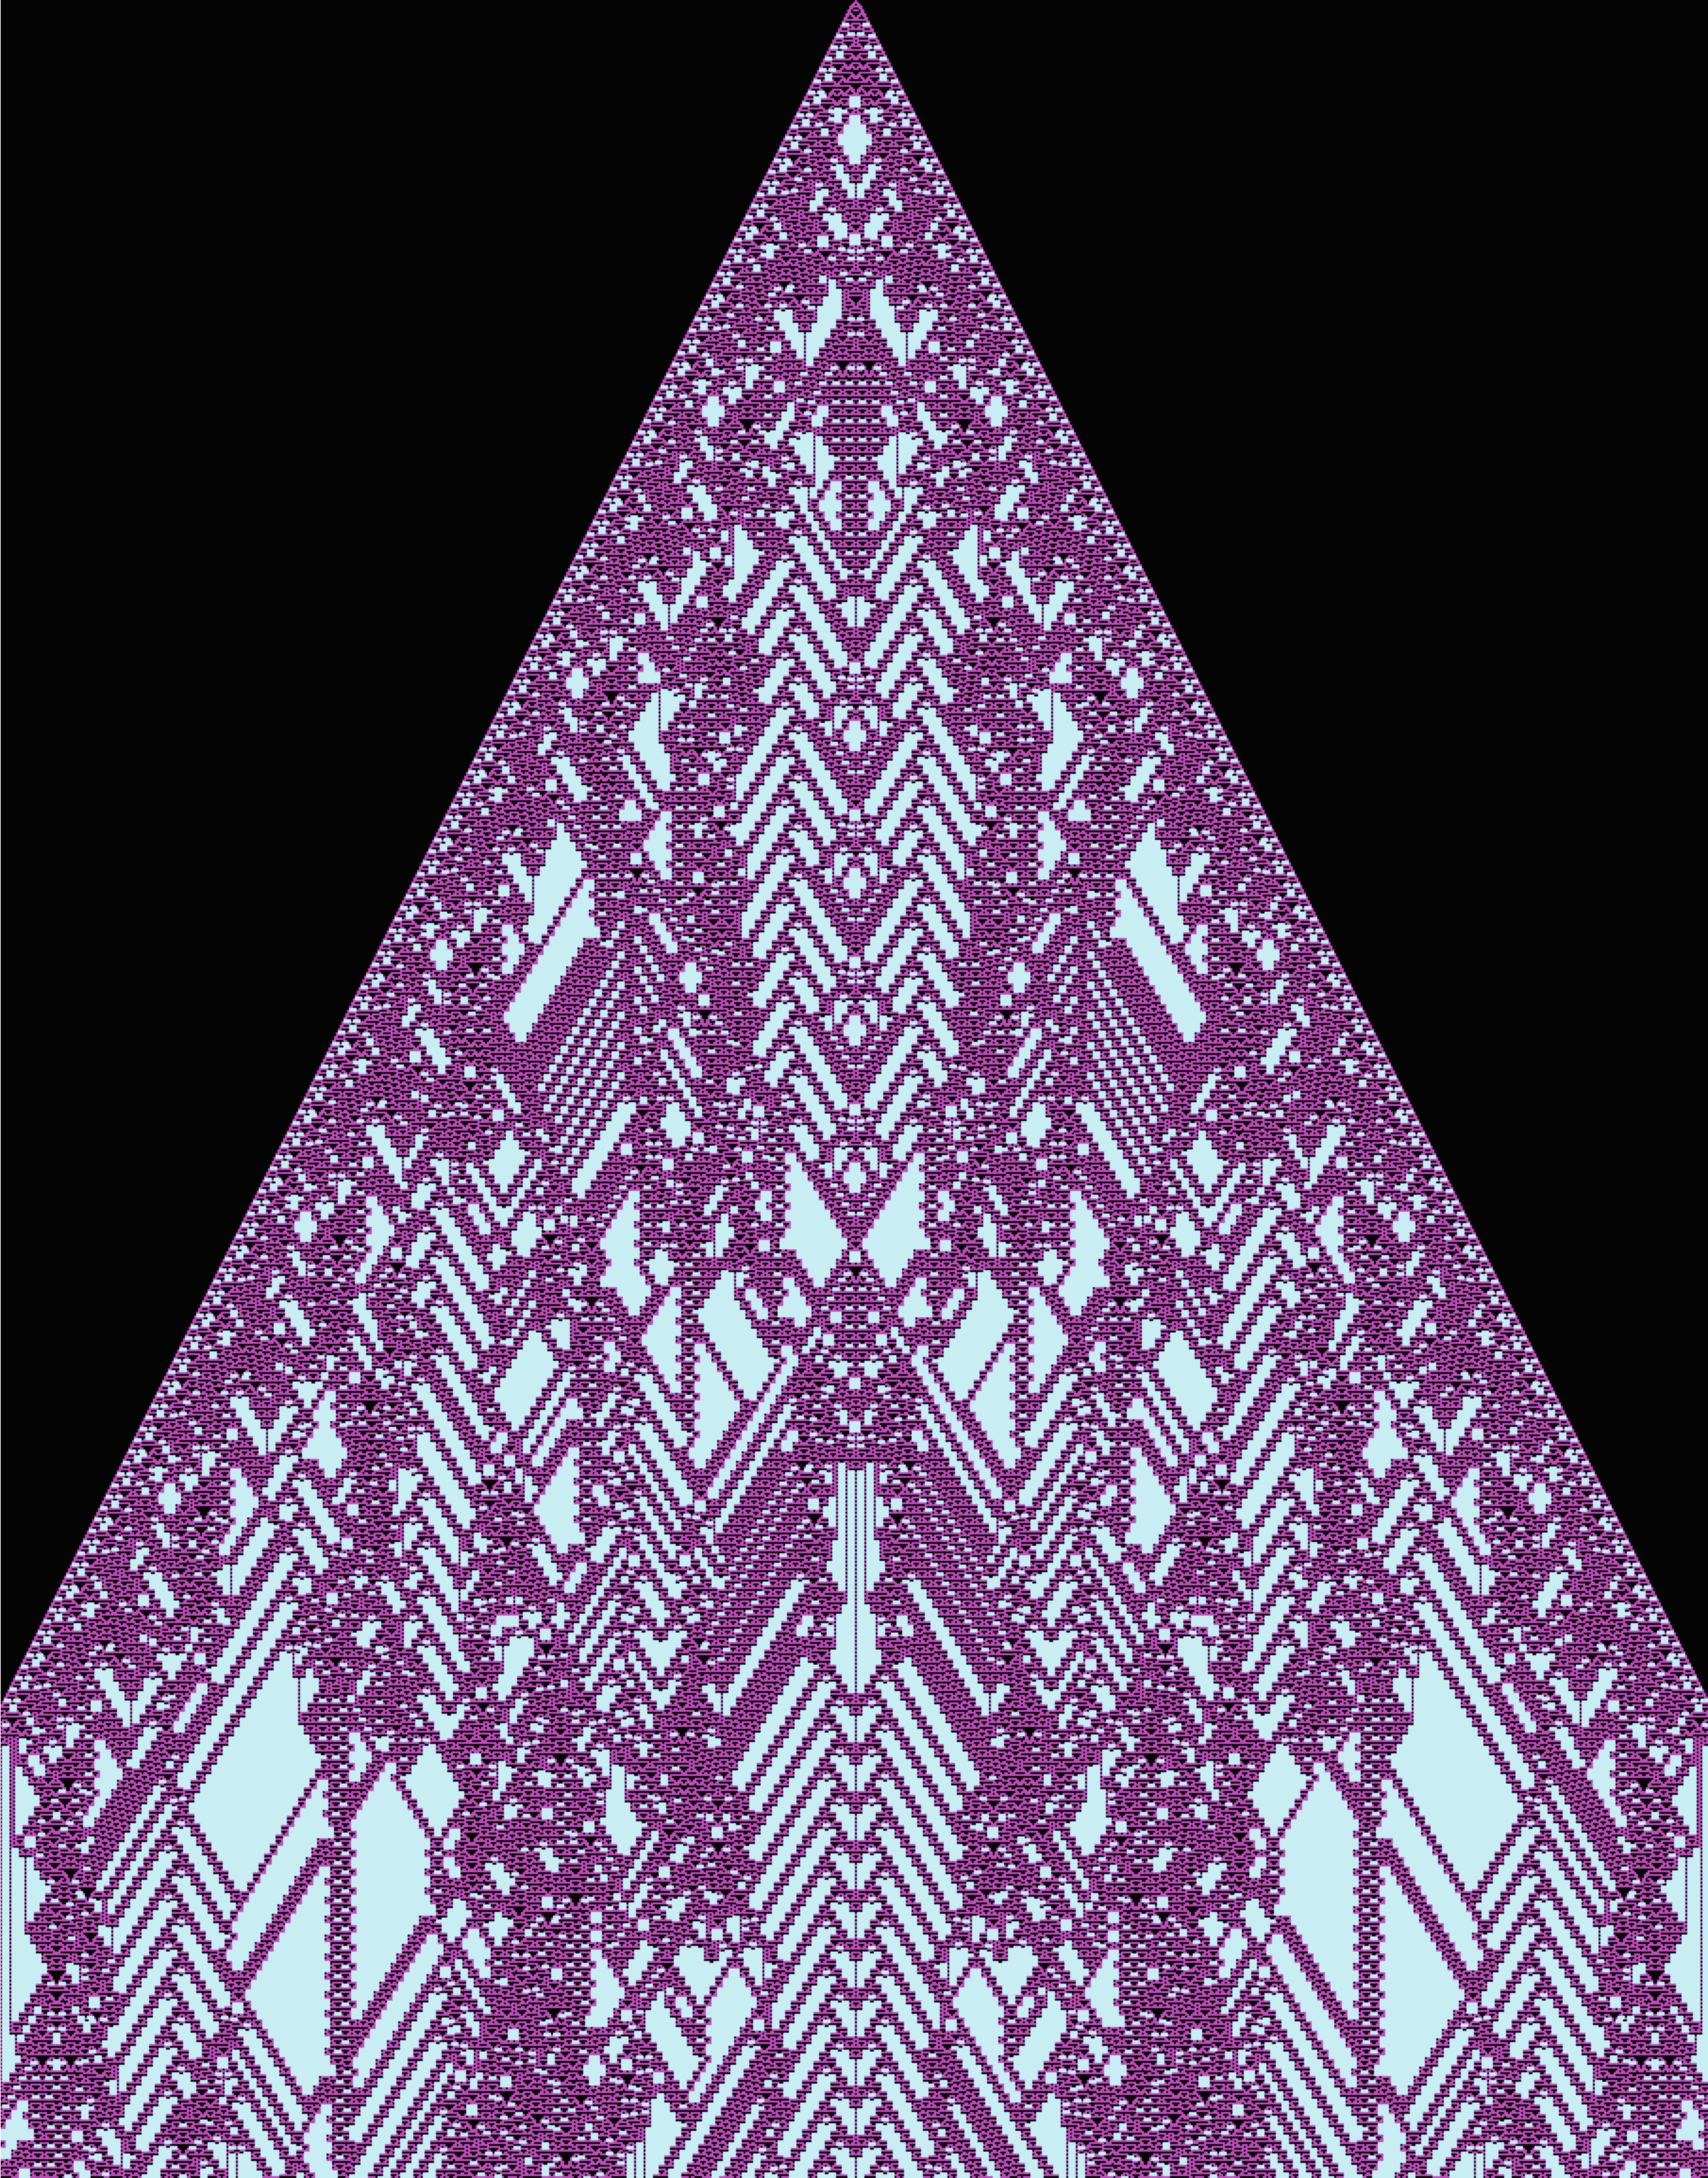
\includegraphics[width=0.4\textwidth]{obrazky-figures/caGliders.png}
    \caption{Obraz Life without Death autora Davida Griffeatha, pro jehož tvorbu bylo upraveno pravidlo automatu Life (vpravo). Obraz Gliders in CA with Memory vytvořen Genarem J. Martinezem, využívající kluzáků (gliders) z automatu Life (vlevo) \cite{CAArt}.}
    \label{fig:caUmeni}
\end{figure}

Generativní a transformativní vlastnosti celulárních automatů využili ve svých bakalářských pracích Mário Gažo \cite{GazoBak} a Martina Zlevorová \cite{ZlevorovaBak} pro transformaci textu. Obě práce jsou inspirovány kolážemi a jsou založeny na rozprostření textu po obrazu. Důležité je, že automaty obou autorů netvoří obraz jako čistě generativní umělecké dílo, ale využívají existujících děl, které obohacují o externí text, nebo rozpoznávají a přemisťují znaky, které se v obrazech již nachází. V obou případech je výsledkem nový obraz -- koláž. Oba autoři využívají u všech efektů pravděpodobnostní tranzitivní funkce s cílem dosáhnout více či méně náhodného rozptylu textu. Výstupy jejich prací jsou znázorněny na obrázku \ref{fig:CAKolaze}.

\begin{figure}[H]
    \centering
    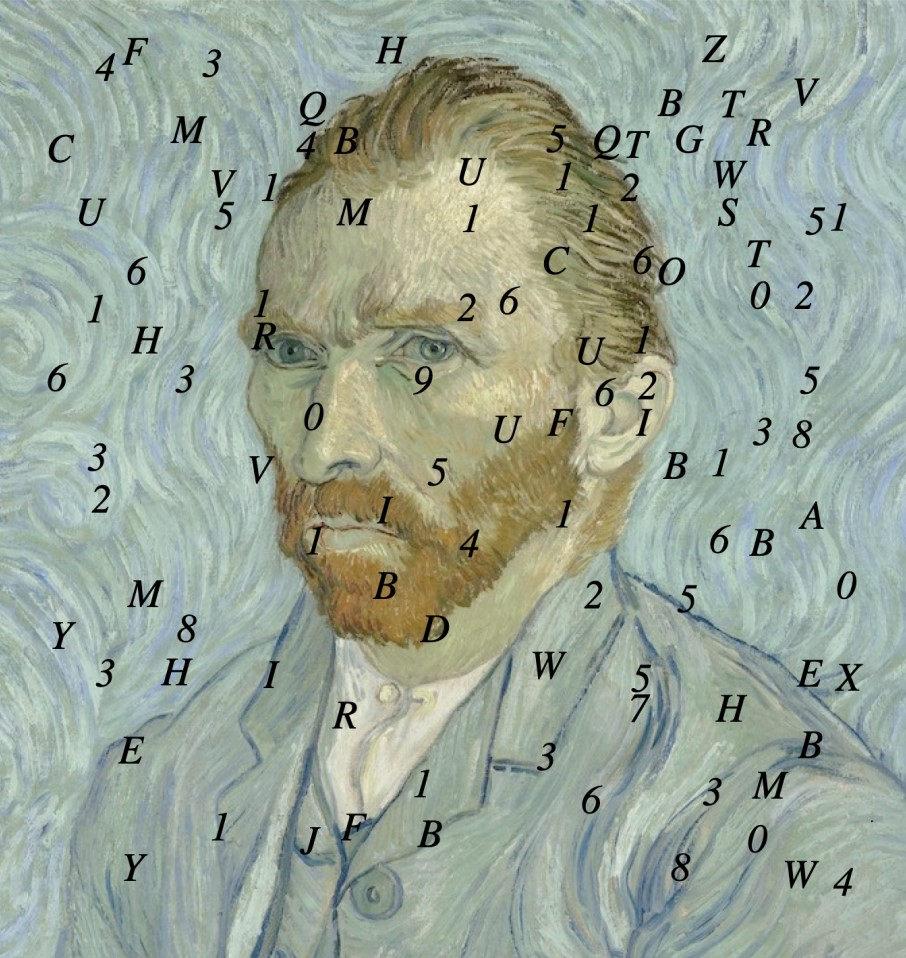
\includegraphics[width=0.4\textwidth]{obrazky-figures/GazoKolaz.jpg}
    \hspace{0.1\textwidth}
    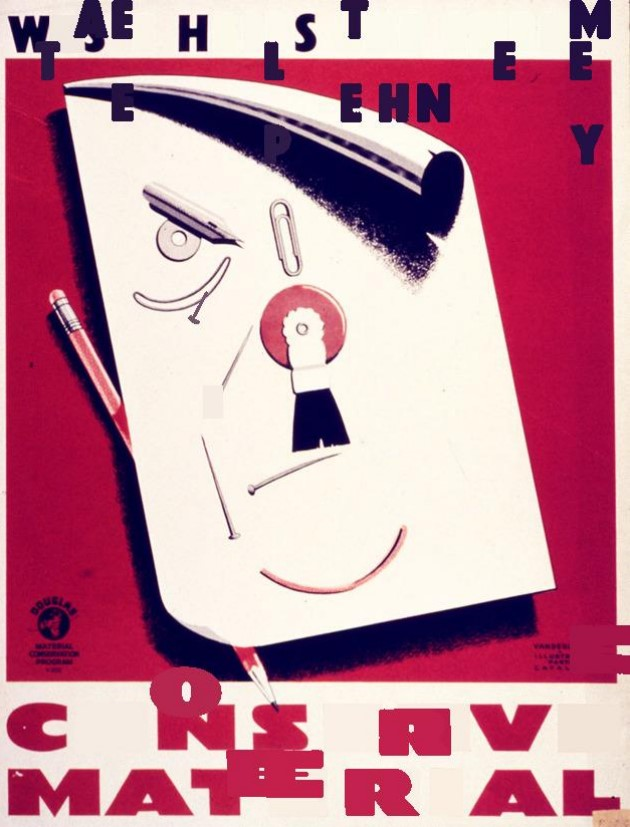
\includegraphics[width=0.4\textwidth]{obrazky-figures/ZlevorovaKolaz.jpg}
    \caption{Koláž autoportrétu Vincenta van Gogha od Mária Gaža (vlevo) \cite{GazoBak} a koláž propagandistického plakátu Martiny Zlevorové (vpravo) \cite{ZlevorovaBak}.}
    \label{fig:CAKolaze}
\end{figure}

\chapter{Automaty navržené pro práci s mřížkou} 
\label{newAutomata}

Tato kapitola se věnuje návrhu modelů, které rozpoznávají vstupní mřížku a provádějí transformace na rozpoznaném poli dlaždic. 

Rozpoznání je rozděleno na čtveřici čtyřcestných automatů, které si vzájemně předávají řízení. Z formálního hlediska má rozpoznání pouze řídící charakter, automaty nejsou samy o sobě schopny mřížku akceptovat, nebo zamítnout, Mezi jejich činností dochází k~modifikacím vstupní mřížky, které je jsou blíže popsány v kapitole \ref{impl}.

Dva celulární automaty popsané v druhé části této kapitoly slouží k vykreslení jednoduchých tvarů, které budou umístěny uvnitř dlaždic, a~k transformaci pole dlaždic tříděním na základě jejich atributů.


\section{Rozpoznání vstupní mřížky}
\label{section:recogTheory}
Termín \emph{mřížka} je z v této práci z pohledu formálních modelů definován jako obraz, který rozděluje plochu na dlaždice.
Na začátku rozpoznání je dána mřížka, která obsahuje pouze tři typy znaků -- hranice dlaždic, prázdný prostor, a hranice obrazu.
Tvar dlaždice musí být z pohledu jejího nejvyššího bodu nejdříve klesající a poté stoupající, s žádnými dalšími změnami, jak je ilustrováno na obrázku \ref{fig:TvaryDlazdic}. Dále se předpokládá, že dlaždice neobsahují díry, t. j. není přípustné, aby se dlaždice nacházela uvnitř dlaždice jiné. Příklady vstupních mřížek jsou uvedeny na obrázku \ref{fig:MrizkaPriklad}. Pokud mřížka splňuje výše definované vlastnosti, je navrženými automaty správně rozpoznána.

Cílem této sekce je navrhnout sérii čtyřcestných automatů, které budou řídit procházení obsahu všech dlaždic mřížky, definované v předchozím odstavci. Záměrem rozpoznání je konceptualizovat mřížku jako dvou-dimenzionálního pole struktur, které představují dlaždice.
\begin{figure}[H]
    \centering
    
\includegraphics[width=\textwidth]{obrazky-figures/tvaryDlazdic.pdf}
    \caption{Příklady povolených a zakázaných tvarů dlaždic v mřížce}
    \label{fig:TvaryDlazdic}
\end{figure}

\begin{figure}[H]
    \centering
    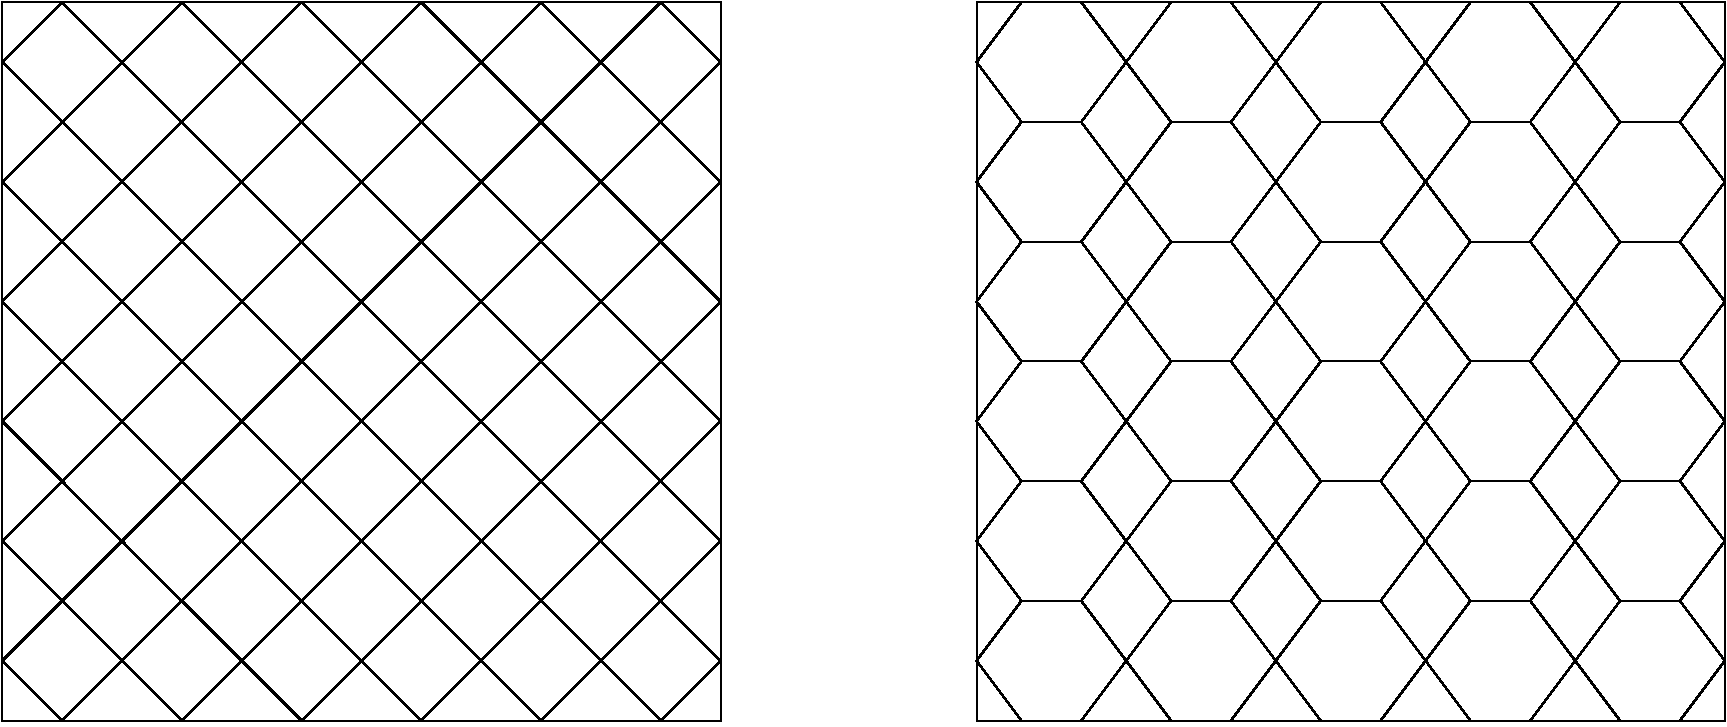
\includegraphics[width=\textwidth]{obrazky-figures/MrizkaPriklad.pdf}
    \caption{Příklady akceptovaných vstupních mřížek, bílá znázorňuje prázdný prostor, černá hranice dlaždic}
    \label{fig:MrizkaPriklad}
\end{figure}

\subsection*{Princip rozpoznání}

Mřížka na vstupu není vyplněná. Rozpoznání provází průběžná výplň dlaždic, na~které automaty při průchodu narazí.

Počátek rozpoznání se nachází v levém horním rohu obrázku, ze kterého je spuštěn automat A1, definovaný v sekci \ref{secA1}, s cílem najít nevyplněný znak uvnitř dlaždice, nacházející se v jejím nejvyšším bodě. V případě, že je nalezen, dojde ke spuštění automatu A2 (\ref{secA2}) a~následně A3 (\ref{secA3}), s cílem obejít konturu dlaždice zevnitř. Dráha opsaná automaty A2 a~A3 se aplikuje formou výplně na prázdné znaky. Po aplikování výplně navazuje svou činností automat A4 (\ref{secA4}), který najde počátek další vrstvy výplně. Postupně jsou přidávány do dlaždice další vrstvy, dokud se zcela nezaplní. Tento postup je proveden na všech dlaždicích, dokud není dosaženo konce mřížky. Proces výplně dlaždice je ilustrován na obrázku \ref{fig:prubehVyplnePOpis}.

\begin{figure}[H]
    \centering
    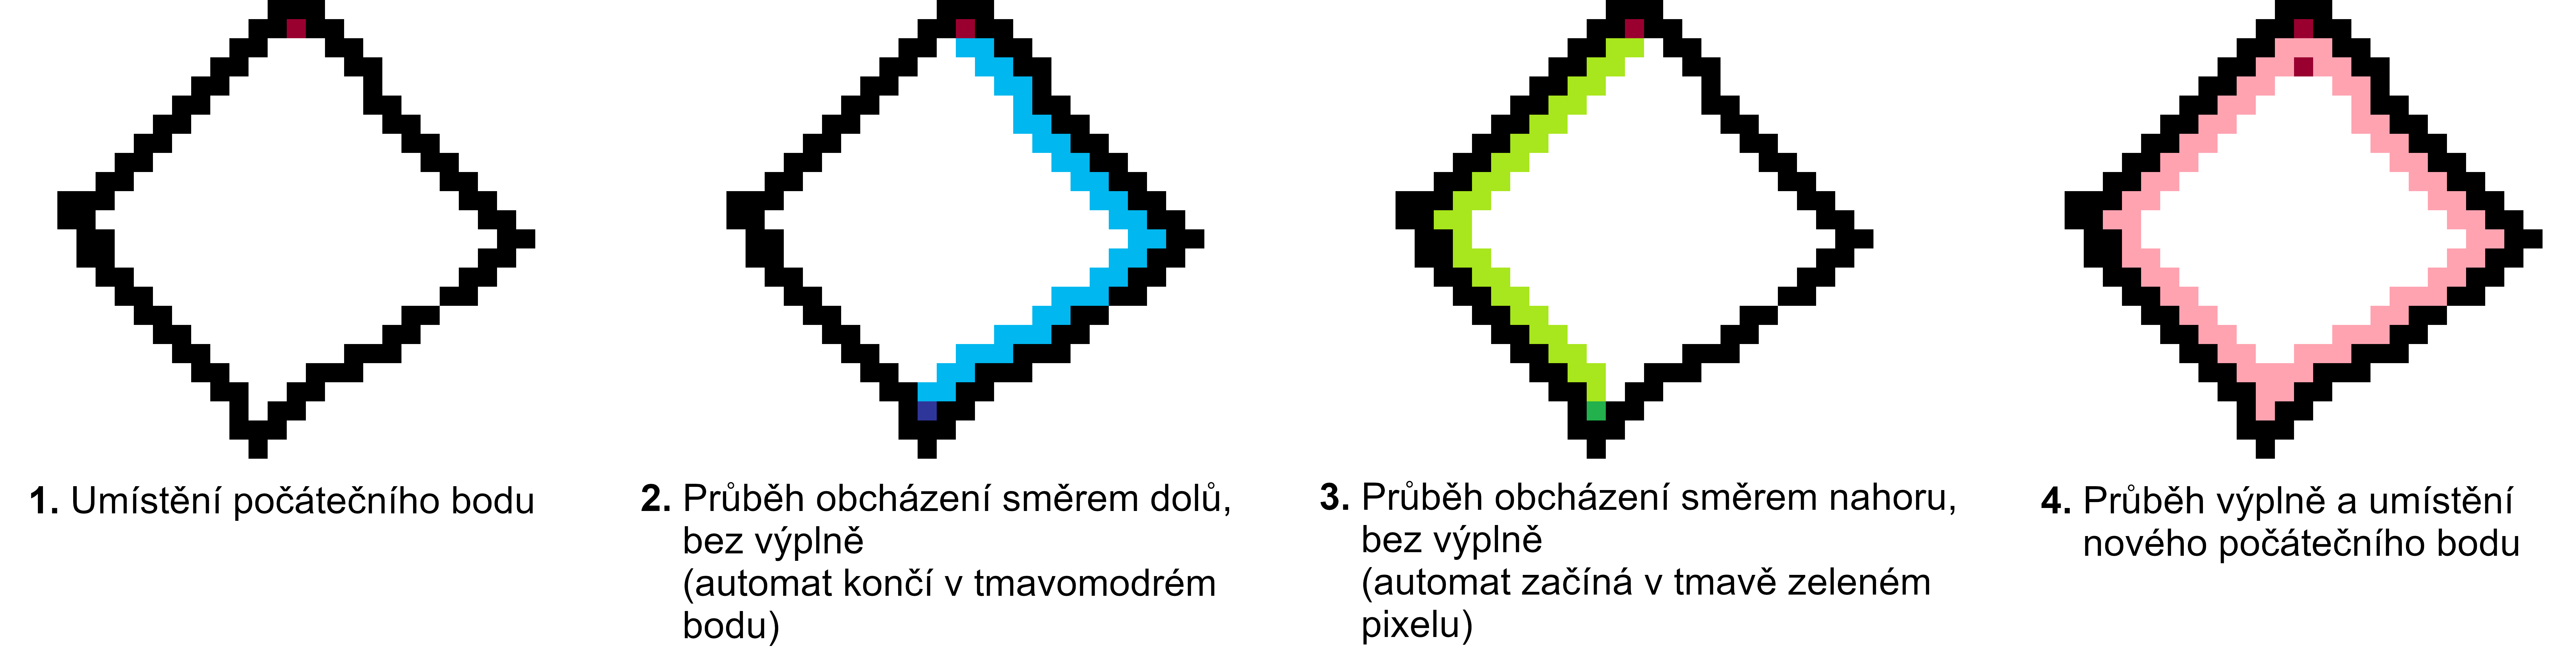
\includegraphics[width=\textwidth]{obrazky-figures/prubehVyplnePopis.png}
    \caption{Ilustrace průběhu výplně jedné vrstvy dlaždice}
    \label{fig:prubehVyplnePOpis}
\end{figure}

\subsection*{Společné definice pro rozpoznávající automaty}

Automaty akceptující mřížku, které budeme v dalších sekcích definovat, sdílejí dvě společné vlastnosti: abecedu $\Sigma$ a množinu povolených směrů $\Delta$. Pro přehlednost a snazší pochopení si společné vlastnosti definujeme v této sekci s tím, že v následujících částech budou automaty specifikovány pouze pomocí diagramu přechodů, s důrazem na proces rozpoznání.

\subsubsection*{Abeceda}

Abeceda $\Sigma = \{\#, B, F, F_{B}, E\}$ má v souvislosti s rozpoznávanou mřížkou následující sémantiku:
\begin{itemize}
    \item $\#$ je znak hranice mřížky (obrazu),
    \item $B$ je znak hranice dlaždice,
    \item $F$ je znak výplně dlaždice,
    \item $F_{B}$ je znak začátku výplně dlaždice,
    \item $E$ je znak prázdného prostoru uvnitř dlaždice.
\end{itemize}

\subsubsection*{Množina povolených směrů}

Množina povolených směrů $\Delta = \{L, R, U, D, N\}$ představuje možnosti pohybu čtecí hlavice čtyřcestných automatů. Znak $N$, který striktně řečeno nepředstavuje směr pohybu, jsem do~množiny přidal, protože dle mého názoru zlepšuje čitelnost diagramu přechodů v situacích, kdy by se automat pohnul jedním směrem, a poté vždy o krok zpět. Automaty stále nazývám jako čtyřcestné, jelikož znak $N$ nějak neovlivňuje volnost pohybu čtecí hlavice. Význam prvků množiny $\Delta$ je popsán níže:

\begin{itemize}
    \item $L$ reprezentuje pohyb doleva,
    \item $R$ reprezentuje pohyb doprava,
    \item $U$ značí pohyb nahoru,
    \item $D$ představuje pohyb dolů,
    \item $N$ reprezentuje absenci pohybu -- čtecí hlavice zůstane na místě.
\end{itemize}

\subsubsection*{Konvence zápisu přechodů}

Diagramy přechodů, které v této kapitole definují čtyřcestné automaty, využívají u popisu přechodů konvenci, popsanou v následujícím odstavci.

Popisy nad šipkami přechodů diagramu jsou definované jako $a \rightarrow d$, kde $a \in \Sigma$,  $d \in \Delta$. Takto je označován přechod, který se provede v situaci, kdy se čtecí hlavice nachází na znaku $a$ a zároveň se posune směrem $d$. Některé přechody jsou zjednodušeně zapsány jako $\rightarrow d$. Takto specifikovaný přechod se provede, pokud nejsou proveditelné žádné nezjednodušené přechody. Z každého stavu může vést nanejvýš jeden zjednodušený přechod.

\subsection*{Automat hledající počátky dlaždic (A1)}
\label{secA1}

Automat definovaný diagramem přechodů na obrázku \ref{fig:PocatkyDlazdic} hledá na vstupní mřížce první prázdný znak v dlaždici. Postupuje shora dolů a zleva doprava tak, aby našel nejvyšší a~nejlevější bod nové dlaždice. Ukončení jeho činnosti ve stavu $S_a$ znamená, že hledání skončilo úspěšně a prázdný znak $E$ je na místě ukončení nahrazen znakem počátku výplně $F_B$. Konec ve stavu $S_r$ naopak značí, že nová dlaždice nebyla nalezena a čtecí hlavice dosáhla konce mřížky.

Tento model jako jediný z navržených využívá skoku na začátek nového řádku, který je blíže popsaný v sekci \ref{skok}. Zavedení skoku vede k jednoduššímu zápisu automatu, který se při sestupu na nový řádek nemusí vracet do nejlevější pozice. Zároveň toto řešení vede k~rychlejšímu průchodu přes řádky obrazu, jelikož stačí každý řádek projít jen jednou. Hledání je ukončeno skokem na znak $\#$.


\begin{figure}[H]
    \centering
    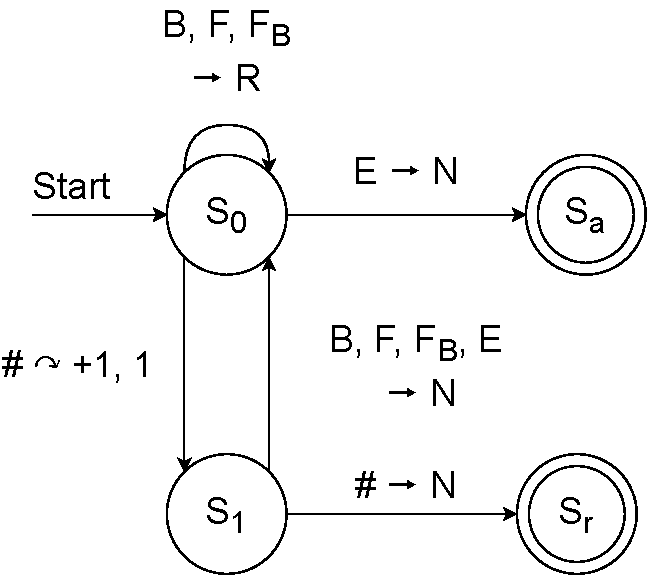
\includegraphics[width=0.4\textwidth]{obrazky-figures/PocatkyDlazdic.pdf}
    \caption{Diagram přechodů automatu, který hledá počátky dlaždic (A1)}
    \label{fig:PocatkyDlazdic}
\end{figure}

\subsection*{Automat obcházející dlaždici směrem dolů (A2)}
\label{secA2}

Smyslem automatu, specifikovaného diagramem přechodů \ref{fig:PoDlazdiciDolu}, je z počátečního bodu $F_B$ zevnitř obejít hranice dlaždice až do chvíle, kdy nebude možné dále pokračovat dolů. Automat se vždy zastaví v nejnižším bodu dlaždice. Princip činnosti můžeme rozdělit do dvou částí. První část, reprezentována stavy $D_0$, $D_1$, $D_2$, a $D_r$, se snaží najít prázdný znak $E$, který by zprava nebo zespodu sousedil s počátečním bodem $F_B$. V případě, že znak není nalezen, je činnost ukončena v zamítajícím stavu $D_r$, jelikož v průchodu není možné pokračovat. V opačném případě se automat snaží posouvat nejprve doprava po hranici a poté dolů. Pokud pohyb směrem dolů není možný, vrací se čtecí hlavice vlevo, dokud znovu nenabyde možnosti posunu dolů. Ukončení nastane dosažením znaku $E$, který je zleva a~zespodu ohraničený znaky $B$ (automat se nemůže posunout vlevo, ani dolů).

\begin{figure}[H]
    \centering
    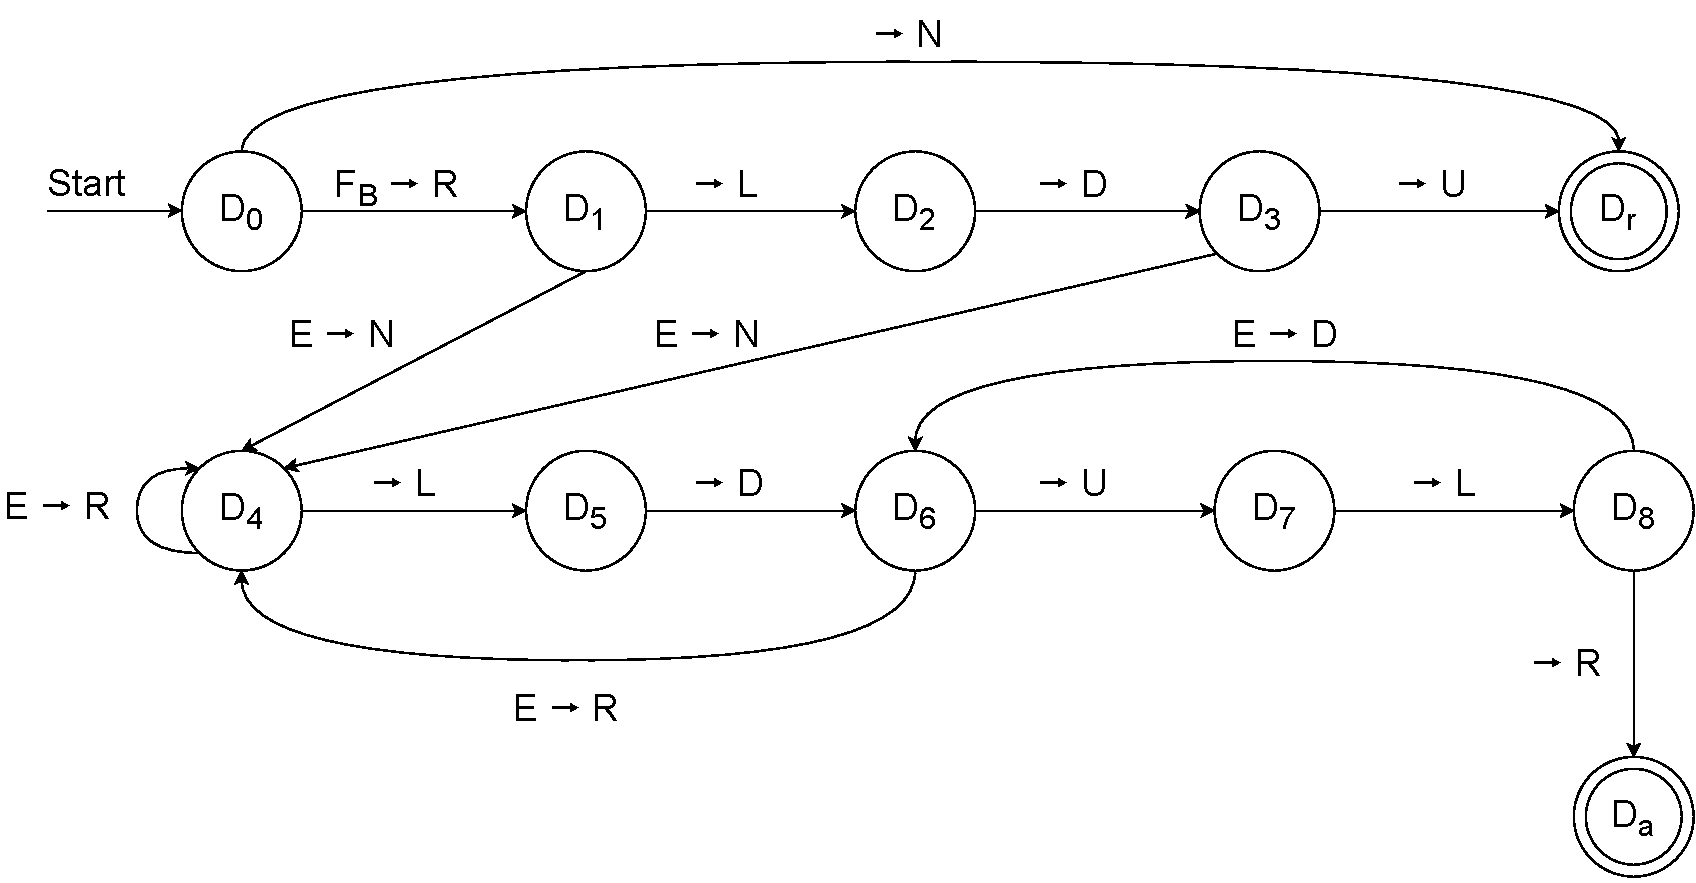
\includegraphics[width=0.9\textwidth]{obrazky-figures/PoBunceDolu.pdf}
    \caption{Diagram přechodů automatu obcházejícího dlaždici směrem dolů (A2)}
    \label{fig:PoDlazdiciDolu}
\end{figure}

\subsection*{Automat obcházející dlaždici směrem nahoru (A3)}
\label{secA3}

Průchod dlaždice směrem nahoru začíná na znaku $E$, kde skončil průchod směrem dolů. Tento automat můžeme chápat jako opačný k automatu A2. Nejprve se čtecí hlavice snaží posouvat po hranici vlevo a poté nahoru. Když směrem nahoru nelze dále pokračovat, snaží se automat vrátit směrem doleva až do chvíle, kdy se znovu může posunout směrem nahoru. Průchod končí dosažením znaku $F_B$, ze kterého byla spuštěna výplň směrem dolů. Automat je definován diagramem přechodů \ref{fig:PoDlazdiciNahoru}.

\begin{figure}[H]
    \centering
    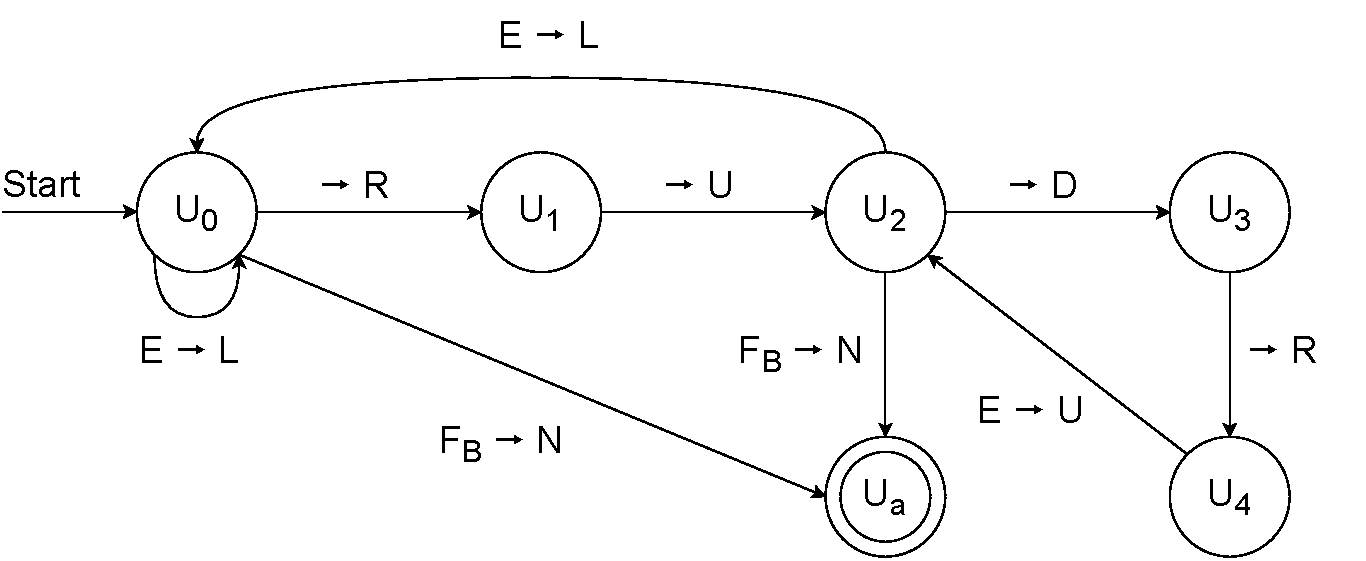
\includegraphics[width=0.9\textwidth]{obrazky-figures/PoBunceNahoru.pdf}
    \caption{Diagram přechodů automatu obcházejícího dlaždici směrem nahoru (A3)}
    \label{fig:PoDlazdiciNahoru}
\end{figure}
\subsection*{Automat hledající nový počátek výplně (A4)}
\label{secA4}

Automat A4 začíná v bodě $F_B$, ze kterého byla spuštěna poslední výplň směrem dolů. Cílem je najít znak $E$ uvnitř průběžně vyplňované dlaždice. Na znak $E$, který automat hledá, jsou kladeny stejné požadavky, jako na první nalezený znak $E$ dlaždice: musí být v~dlaždici nejvýše položený a co nejvíce vlevo. Automat začíná z počátečního bodu posunem doprava do stavu $N_1$. Předpokládáme, že se nenachází žádný znak $E$, který by ležel nahoře, nebo vlevo relativně k bodu, na kterém automat spustil činnost. Pokud je dosaženo znaku $E$, je hledání ukončeno jako úspěšné a na místo znaku $E$ je vložen znak $F_B$. V opačném případě dojde k posunu na další řádek směrem dolů. Na dalším řádku se čtecí hlavice nejprve vrátí k nejlevějšímu hraničnímu znaku a poté znovu ve stavu $N_1$ hledá znak $E$. Pokud stavové řízení sestoupí dolů a na dalším řádku se nachází znak hranice dlaždice $B$, dojde k posunu směrem doleva, dokud na následujícím řádku automat nenarazí na znak $F$ nebo $E$. Pokud je zleva dosaženo znaku $B$, ukončí se vyhledávání zamítacím stavem $N_r$, jelikož tímto automat došel na konec dlaždice.

\begin{figure}[H]
    \centering
    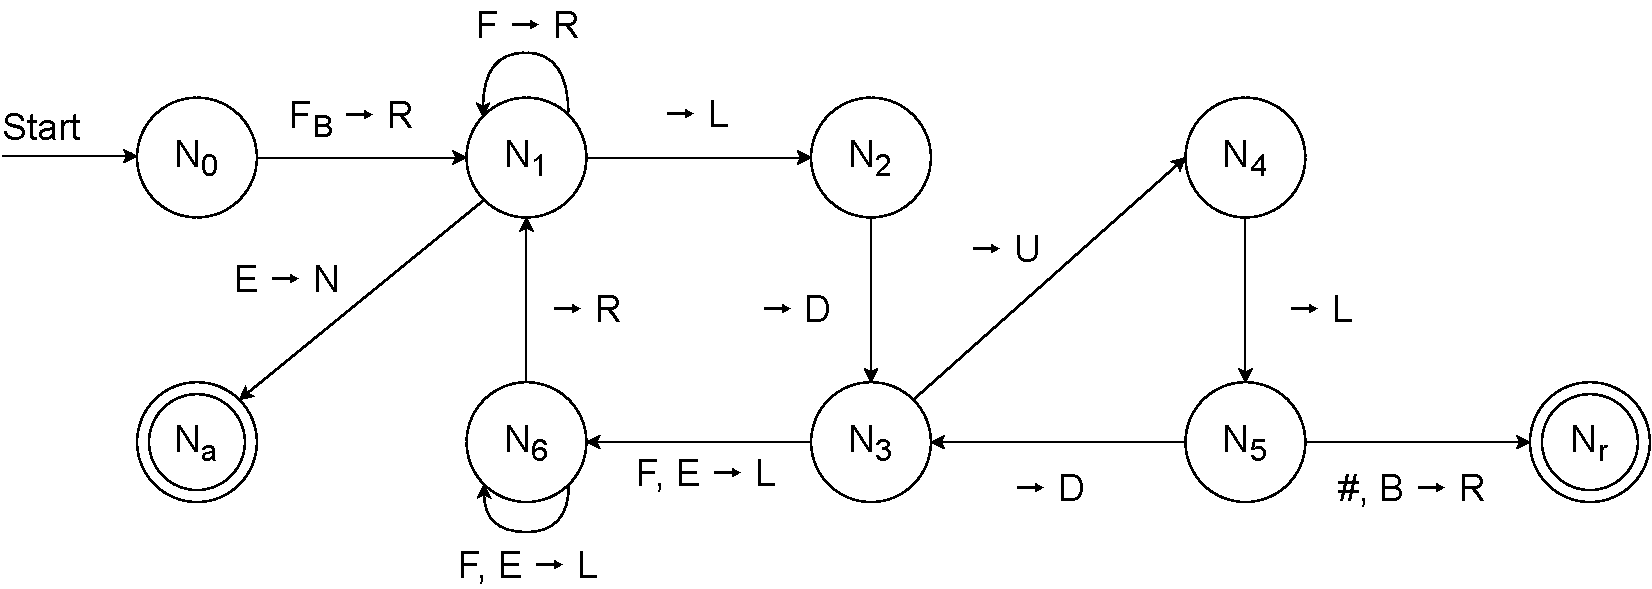
\includegraphics[width=0.9\textwidth]{obrazky-figures/NovyPocatek.pdf}
    \caption{Diagram přechodů automatu, který hledá nový bod výplně (A4)}
    \label{fig:Novy pocatek}
\end{figure}

\section{Uspořádání 2D pole dlaždic}
\label{section:sortingCA}

Rozpoznání mřížky končí umístěním dlaždic do abstraktní datové struktury, kterou si pro potřeby této sekce konceptualizujeme v souladu s definicí celulárního automatu jako dvou-dimenzionální pole buněk, které se mohou nacházet v určitých stavech. V této sekci budeme dlaždice nazývat jako buňky a jejich vlastnosti jako stavy. Na vstupu celulárního automatu je pole buněk s náhodně vybranými (neuspořádanými) stavy. Cílem automatu, navrženého v této části, je tyto buňky uspořádat podle určitých kritérií. Dílčí aspekty celulárního automatu budou v této sekci popsány prostřednictvím datových struktur (stavů) a procedur (tranzitivních funkcí).

\subsection*{Stavy}
Stav buňky sestává z jednotlivých atributů, které mohou nabývat hodnot nezávisle na sobě, a společně tvoří stav.
Stav
$$s = (Size, Shape, ShapeColorIntensity, BackgroundColorIntensity)$$ 
má následující význam atributů:

\begin{itemize}
    \item $Size$ je celé číslo, které představuje velikost tvaru uvnitř buňky.
    \item $Shape$ je typ vnitřního tvaru dlaždice, který může nabývat jedné z následujících hodnot: $\{RotatedSquare, Square, TrianglePointedUp, TrianglePointedDown\}$.
    \item $ShapeColor$ je barvou vnitřního tvaru dlaždice.
    \item $BackgroundColor$ představuje barvu pozadí dlaždice.
\end{itemize}

\subsection*{Tranzitivní funkce}
Tranzitivní funkce programu mění stav buněk v Mooreově okolí $(r = 1)$. Na vstupu tranzitivní funkce je seznam řídících argumentů, které udávají, jakým způsobem bude měnit stav buněk v okolí. Stav okolí $n$ je seznam stavů jeho dílčích buněk. Pro popis jednotlivých buněk v okolí je využita konvence uvedená na obrázku \ref{fig:CAOkoli}. Lokální tranzitivní funkci definujeme jako:

$$\delta(d_{size}, d_{background}, d_{foreground}, f_{type}, n_{current}) = n_{next} $$ 

kde $d_{size}, d_{background}, d_{foreground} \in D \cup \{n\}$, přičemž $n$ představuje situaci, kdy není vybrána buňka k porovnání. Množina $D = \{u, d, l, r, ur, ul, dr, dl\}$ představuje relativní souřadnice sousedních buněk vůči centrální buňce.   Argument $f_{type} \in F$, $F = \{true, false\}$ značí, zda bude aplikována transformace na základě typu vnitřního tvaru buňky. Symboly $ n_{current}, n_{next} \in S$, kde $S$ je množinou všech stavů okolí, udávají současný a následující stav okolí. Význam symbolů v zápisu tranzitivní funkce je definován jako:

\begin{itemize}
    \item $d_{size}$ značí relativní souřadnice sousední buňky, se kterou je porovnána centrální buňka na základě jejich velikostí $(Size)$.
    \item $d_{background}$ specifikuje umístění buňky z okolí, se kterou je porovnána centrální buňka dle barvy pozadí $(BackgroundColor)$.
    \item $d_{foreground}$ má stejnou sémantiku jako symbol výše, akorát uvažuje barvu vnitřního tvaru $(ShapeColor)$.
    \item $f_{type}$ značí, zda dojde k výměně buněk v okolí na základě vnitřního tvaru buňky.
    \item $n_{current}$ představuje vstupní okolí.
    \item $n_{next}$ představuje výstupní okolí.
\end{itemize}

Tranzitivní funkce na základě vstupů vytváří uspořádání v okolí. Podstatné je, že uspořádání vždy probíhá pouze po dílčích atributech, a nikdy tak nedojde k výměně celého stavu buňky; může být však vyměněno více atributů najednou. Pro argumenty, udávající vybrané sousední buňky z množiny $D$ platí, že pokud se rovnají symbolu $n$, tak se dané uspořádání neprovede, jelikož není dána buňka k porovnání. V případě, že buňka vybraná pro porovnání přesahuje hranice pole dlaždic, taktéž nedojde k výměně. Uspořádání, které podporuje definovaná tranzitivní funkce, jsou popsány níže a znázorněny na obrázku \ref{fig:usporadani}.

\subsubsection*{Uspořádání na základě velikosti}

Pokud je sousední buňka specifikovaná v parametru $d_{size}$ menší, než centrální buňka, dojde k prohození jejich atributů $Size$.

\subsubsection*{Uspořádání na základě typu vnitřního tvaru}


Každý tvar má pevně definovaný pohyb: čtverce se posouvají doleva, kosočtverce doprava, trojúhelníky se špičkou otočenou nahoru se posouvají výše, a trojúhelníky otočené špičkou dolů se pohybují po obrazu dolů. Pohyb je aplikován pokud pro atribut $f_{type}$ platí: $f_{type} = True$. Výměna je realizována prohozením atributů $Shape$.

\subsubsection*{Uspořádání na základě barvy pozadí}

Pokud je barva pozadí sousední buňky daná argumentem $d_{background}$ světlejší, než barva pozadí centrální buňky, prohodí se jejich atributy $BackgroundColor$.

\subsubsection*{Uspořádání na základě barvy vnitřního tvaru}

V případě, že je barva vnitřního tvaru sousední buňky specifikovaná parametrem $d_{foreground}$ světlejší, než barva vnitřního tvaru centrální buňky, dojde k výměně atributů $ShapeColor$.

\begin{figure}[H]
    \centering
    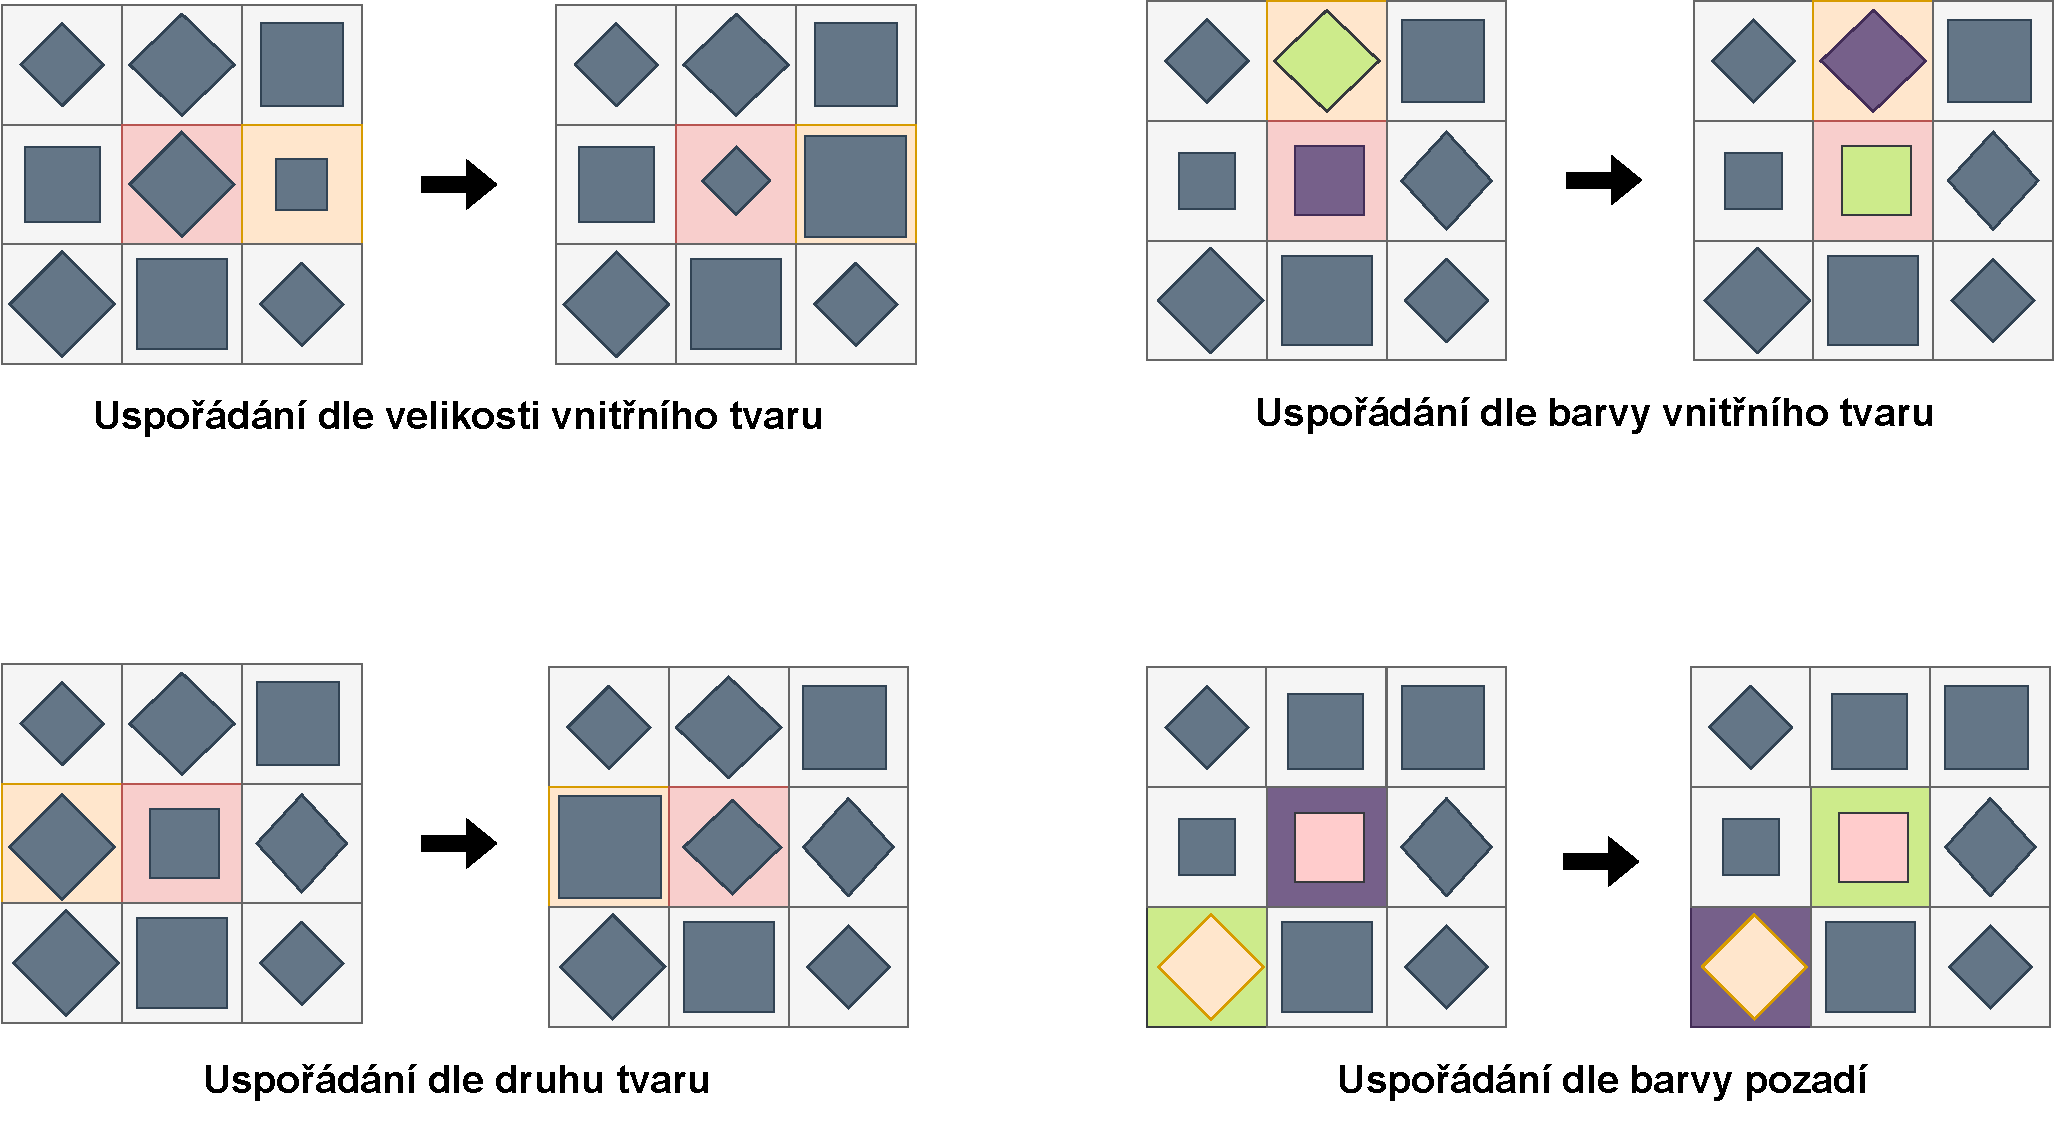
\includegraphics[width=\textwidth]{obrazky-figures/Usporadani.pdf}
    \caption{Ilustrace uspořádání definovaných tranzitivní funkcí. Světle červenou je znázorněna centrální buňka, sousední buňka je vybarvena světle oranžovou.}
    \label{fig:usporadani}
\end{figure}

\section{Tvorba vnitřních tvarů dlaždic}
\label{section:GrowingCA}
Vnitřní tvary dlaždic jsou vykresleny pomocí jednoduchého celulárního automatu. Růst tvarů probíhá na dvou-dimenzionálním poli buněk, které je odděleno od dlaždic a mřížky. Proces přenesení vykreslených tvarů do dlaždic je popsán v kapitole \ref{impl}. Vstupní konfiguraci představuje pole prázdných buněk s jednou zaplněnou buňkou ve středu. Buňky mohou nabývat pouze dvou stavů: prázdná a plná. Typy vykreslených tvarů se liší pouze na základě okolí, která jsou definována na obrázku \ref{fig:VnitrniTvar}. Tranzitivní funkce je pro všechna okolí definována stejně: pro každou buňku $S$, která je vyplněná, se vyplní všechny buňky jejího okolí. Růst tvaru je znázorněn na příkladu s trojúhelníkem, který reprezentuje obrázek \ref{fig:RustTvaru}. 

\begin{figure}[H]
    \centering
    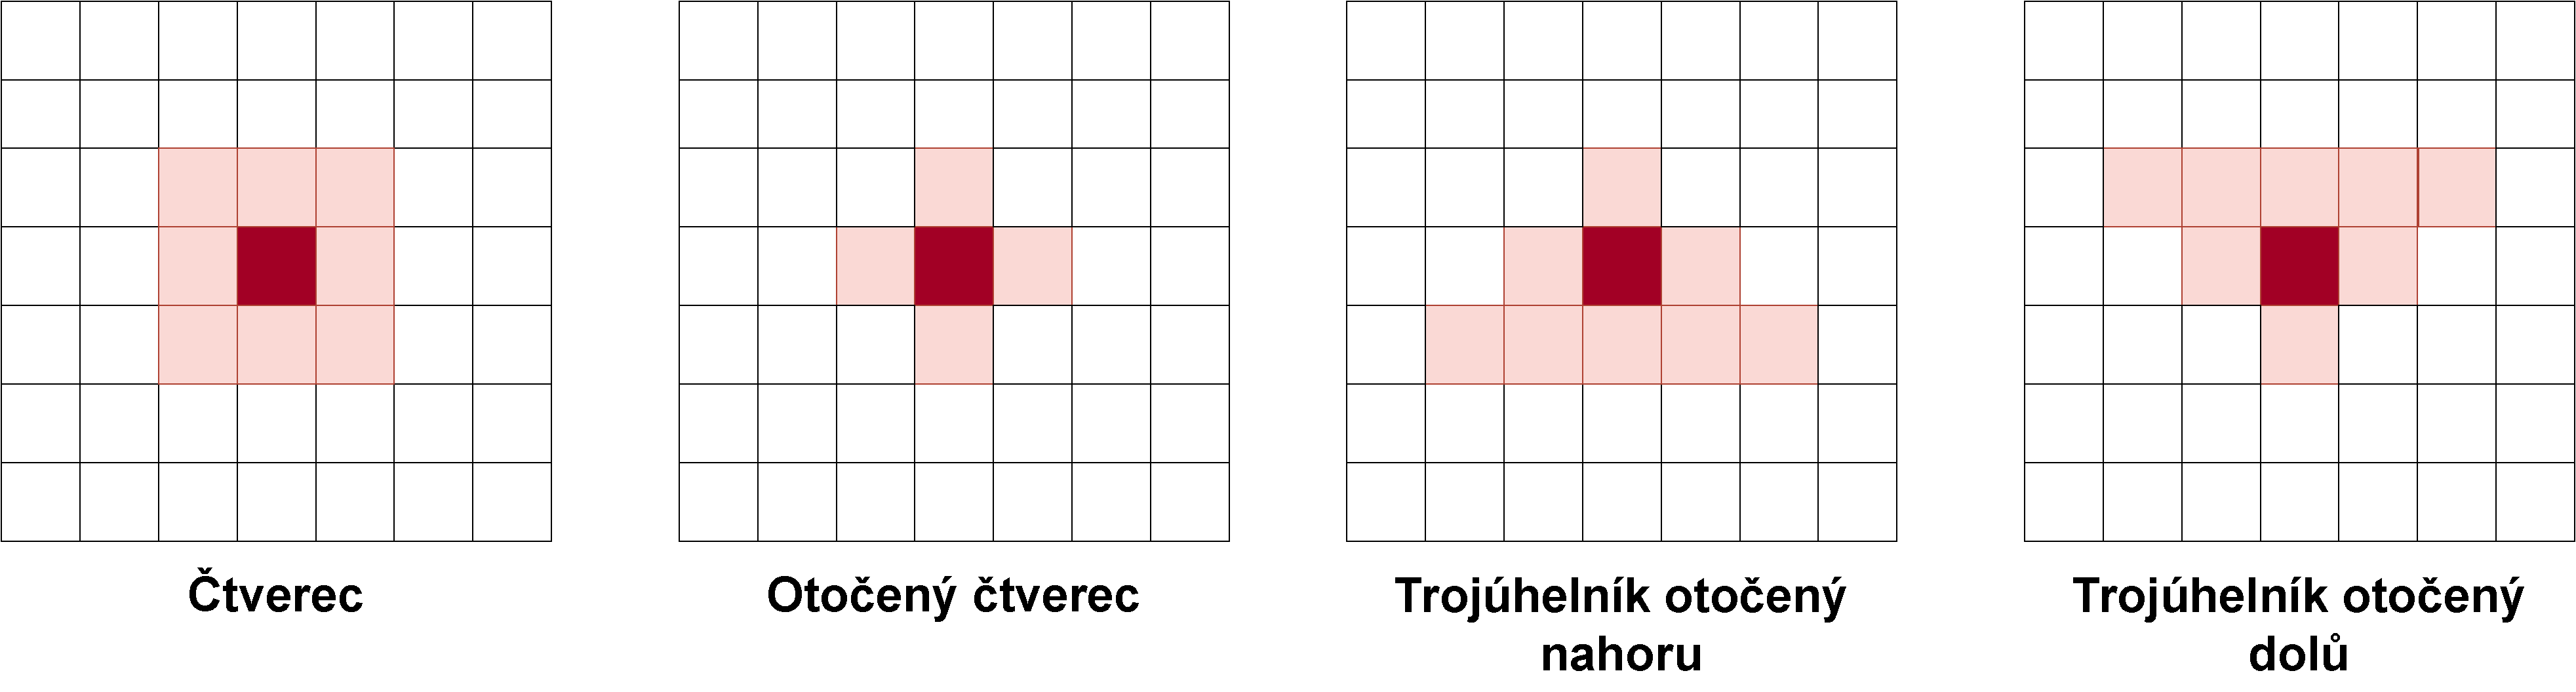
\includegraphics[width=0.9\textwidth]{obrazky-figures/VnitrniTvar.pdf}
    \caption{Podporované druhy okolí automatu produkujícího výplňové tvary dlaždic}
    \label{fig:VnitrniTvar}
\end{figure}

\begin{figure}[H]
    \centering
    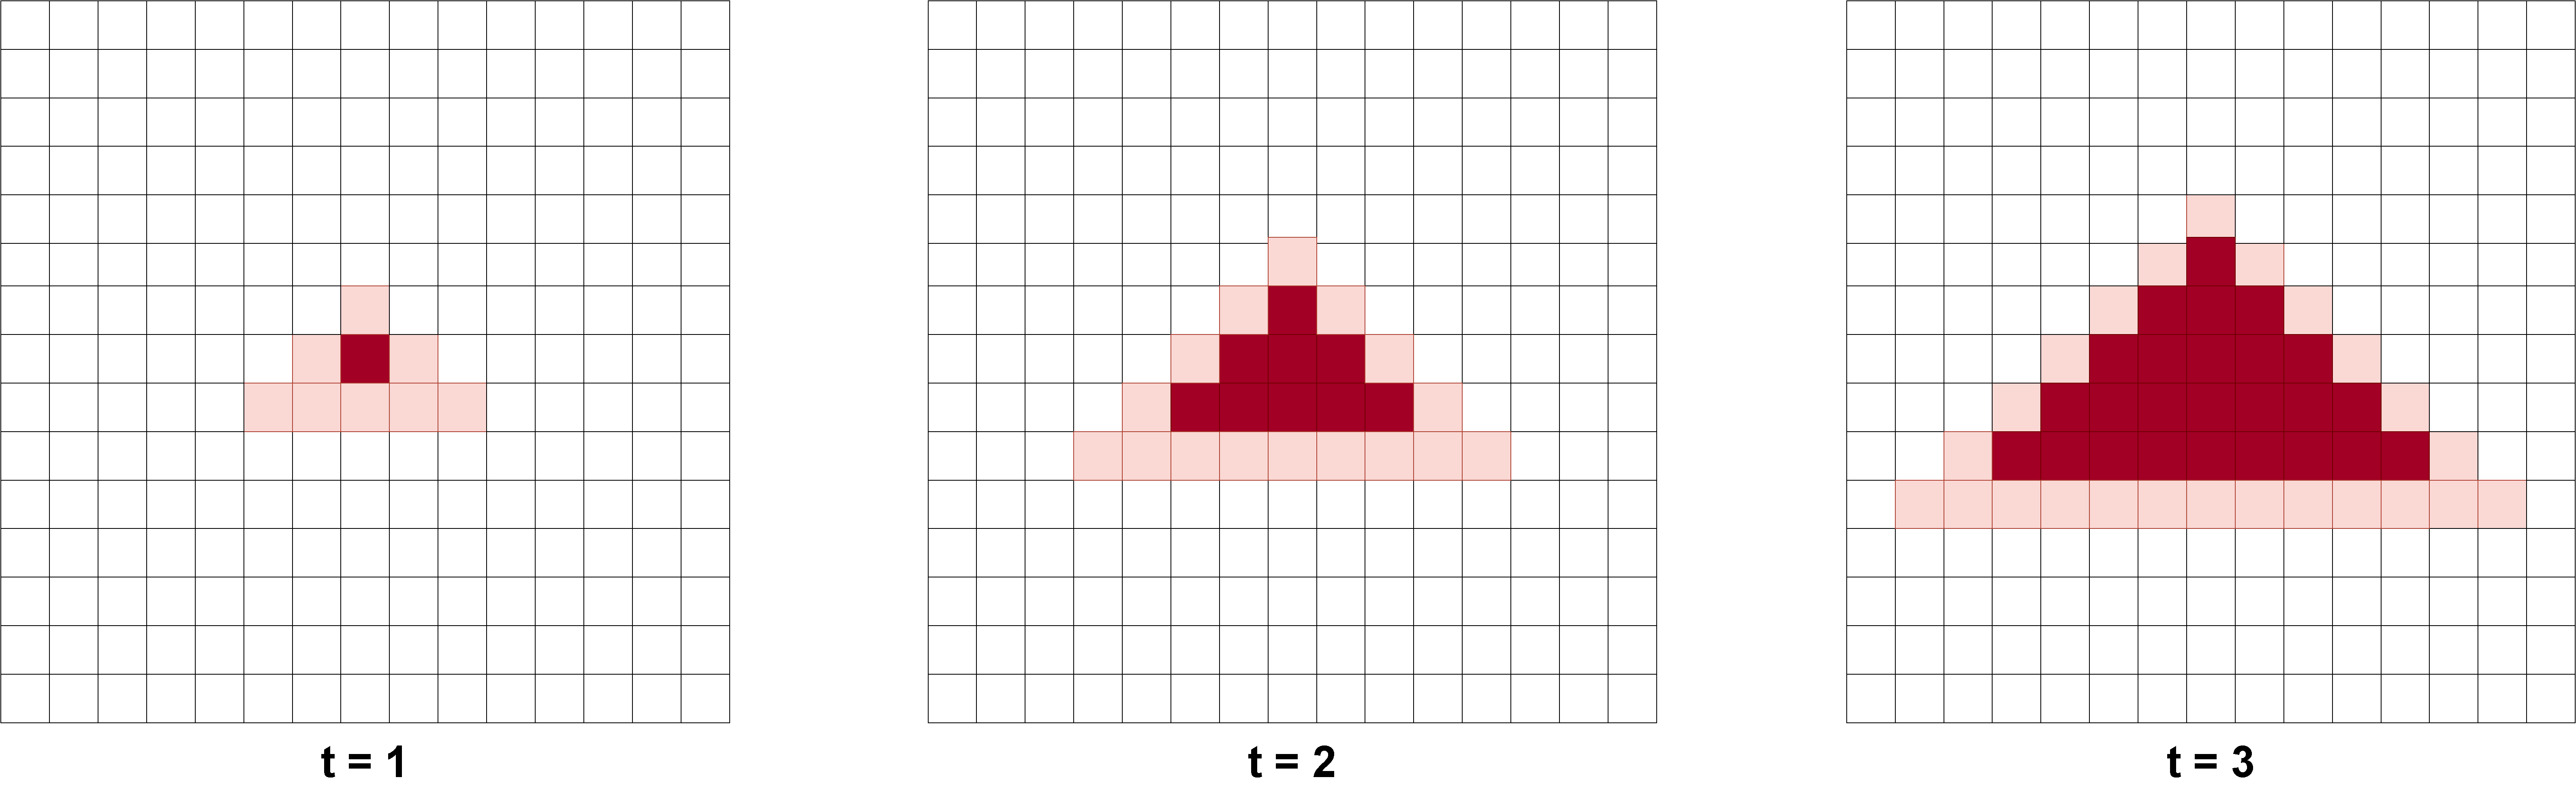
\includegraphics[width=0.9\textwidth]{obrazky-figures/RustTvaru.pdf}
    \caption{Příklad průběhu růstu tvaru na trojúhelníkovém okolí}
    \label{fig:RustTvaru}
\end{figure}

\chapter{Implementace rozpoznání a transformace mřížky} 
\label{impl}

Tato kapitola se věnuje návrhu a implementaci aplikace, která využívá modely navržené v~předchozí kapitole jako formální základ pro rozpoznání a transformaci vstupní mřížky. Navržený program zpracuje vstupní mřížku, kterou specifikuje uživatel, do výstupního videa. Krátký klip, který je z mřížky vytvořen, se skládá ze snímků obsahujících obarvené dlaždice s vnitřními tvary. Jednotlivé snímky reprezentují konfigurace celulárního automatu, který nad polem dlaždic provádí transformace. Výsledkem je tak vizualizace průběžného uspořádání dlaždic dle jejich vlastností. 

V následujících sekcích je implementace nejprve blíže popsána z hlediska použitých technologií a z vysokoúrovňového pohledu na její procedurální strukturu. Aplikace je implementována jako modulární, a proto v další části popisu implementace na program nahlížíme po~jednotlivých modulech, které jsou blíže rozebrány.
\section{Použité nástroje}
\label{impl:utils}
Pro implementaci programu jsem zvolil interpret Python verze 3.10 \cite{python}. Rozhodl jsem se tak zejména kvůli tomu, že obsahuje několik knihoven užitečných pro tuto práci. Knihovny potřebné pro spuštění jsou popsány níže.

\begin{itemize}
    \item \verb|cv2| je knihovna počítačového vidění, v tomto projektu je využita pro načítání a zpracování obrazu a pro výstup ve video formátu \cite{cv2}.
    \item \verb|numpy| definuje datové struktury, do kterých knihovna \verb|cv2| ukládá obraz \cite{numpy}.
    \item \verb|extcolors| slouží pro extrakci barev z obrazu \cite{extcolors}.
\end{itemize}

\section{Popis použití}

Program je implementován jako konzolová aplikace, která vyžaduje povinné argumenty ale zároveň nabízí sadu volitelných vstupů, které dávají uživateli prostor s programem experimentovat pro dosažení různých výsledků. Níže stručně popíšu spuštění programu. Detailnější popis argumentů je k dispozici spuštěním programu s přepínačem \verb|-h|.

\begin{quote}
    \verb|auto-vasarely [-h] [-b PATH] [-c PATH] [-s SHAPES]| \linebreak
    \verb|[-n NUMBER_OF_TRANSFORMATIONS] [-st] [-ss DIRECTION]| \linebreak
    \verb|[-lb DIRECTION] [-ls DIRECTION] [-o SCALE] [-jt]| \linebreak
    \verb|grid_path row_sequence background_colors_path output_path| \linebreak
\end{quote}

Povinné argumenty jsou celkem čtyři. První dva specifikují cestu k~obrazu, který reprezentuje mřížku, a sekvenci délek řádků zapsaných jako číslice oddělené pomlčkou (např.: sekvence \verb|5-2| reprezentuje opakující se řádky o délce 5 a délce 2). Následují dva povinné argumenty, udávající cestu k barevnému obrazu, který bude převeden na paletu, a cestu k~výstupní složce, ve které bude uloženo video.

Volitelné argumenty jsou znázorněny pomocí hranatých závorek. Argumenty  \verb|-b| a \verb|-c| specifikují cestu k obrázkům, kde první obsahuje barvu hraničních pixelů dlaždic a druhý barvu vnitřních tvarů. Pomocí argumentu \verb|-s| můžeme zvolit, jaké typy vnitřních tvarů chceme do~dlaždic přidat. Argument \verb|-n| specifikuje počet provedených transformací a výstupních konfigurací. Způsob transformace specifikujeme pomocí sady argumentů \verb|-ss|, \verb|-lb|, a \verb|-ls|, které mění směr pohybu atributů dlaždic, a přepínače \verb|-st|, díky kterému jsou transformace aplikovány na základě typu vnitřního tvaru. Argument \verb|-o| definuje zvětšení či zmenšení rozlišení výstupu relativně k rozlišení načtené mřížky. Přepínač \verb|-jt| způsobí, že se uloží jen první a~poslední konfigurace celulárního automatu.

\section{Struktura aplikace}

Aplikace je z procedurální stránky navržena dle obrázku \ref{fig:Structure}. Nejprve je zpracována vstupní mřížka, která je následně rozpoznána jako pole dlaždic. Následuje konverze referenčních obrazů do barevných palet a inicializace pole dlaždic. Poté je proveden počet transformací, který je zvolen uživatelem. Výsledné konfigurace jsou uloženy, a nakonec konvertovány do~video výstupu.

\begin{figure}[H]
    \centering
    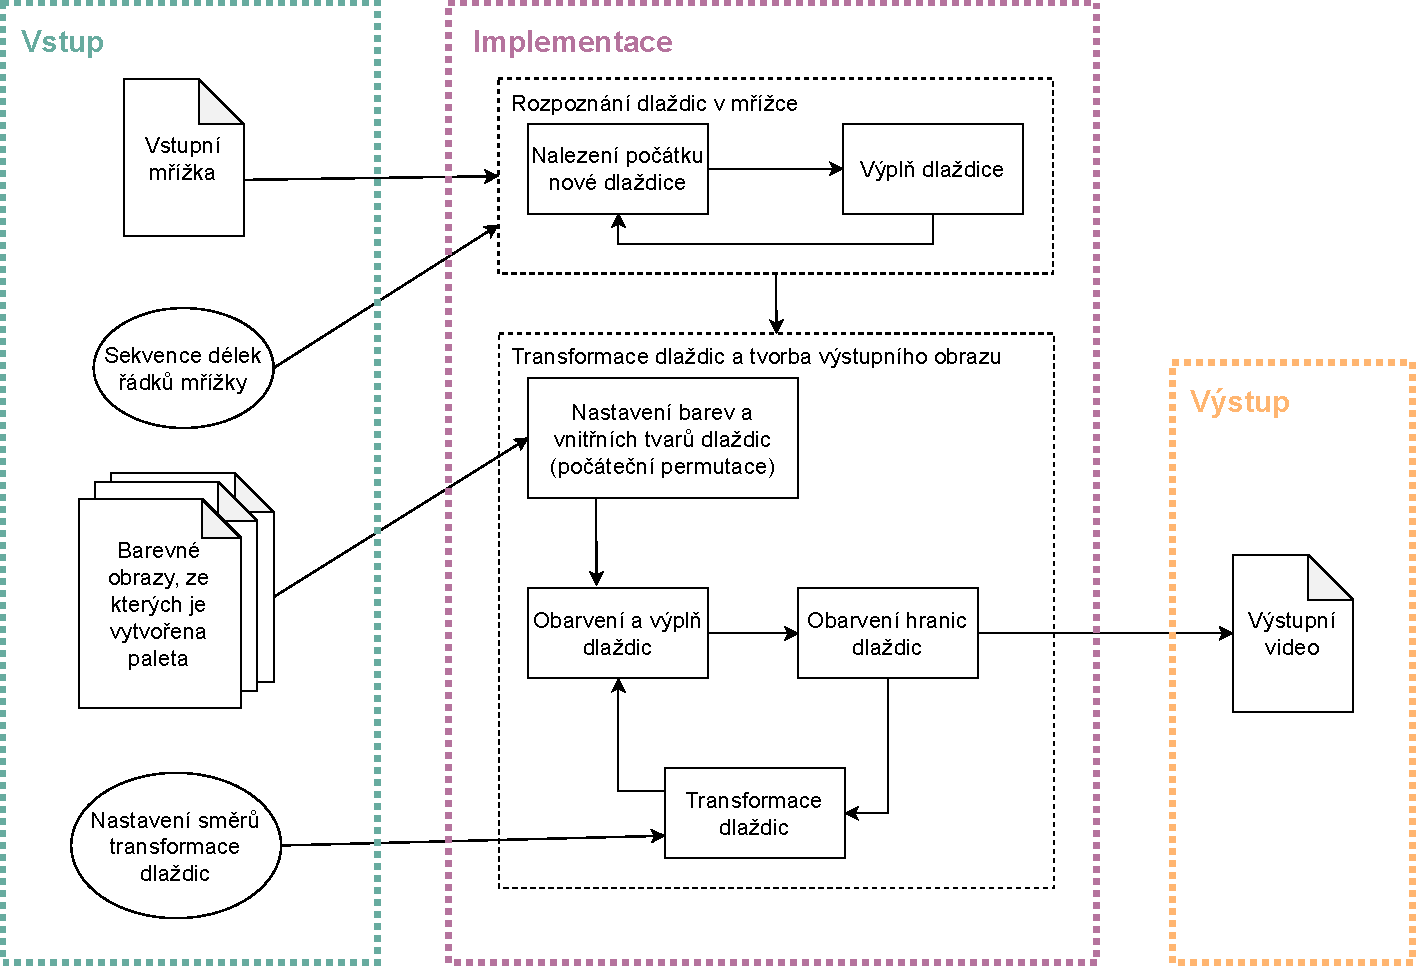
\includegraphics[width=\textwidth]{obrazky-figures/StrukturaAplikace.pdf}
    \caption{Struktura aplikace z procedurálního pohledu}
    \label{fig:Structure}
\end{figure}

Program je složen s dílčích modulů, které obsahují implementace datových struktur, poskytujících abstraktní pohled na mřížku, a procedur, které zajišťují její rozpoznání a~zpracování. Ve výčtu níže jsou moduly stručně popsány.

\begin{itemize}
    \item \verb|auto_vasarely.py| je vstupním bodem aplikace, zajišťuje zpracování argumentů příkazové řádky. Volá funkce ostatních modulů v procedurální posloupnosti dle obrázku \ref{fig:Structure}.
    \item \verb|parser.py| zajišťuje zmenšení obrázku a jeho konverzi na mřížku, kterou jsou navržené čtyřcestné automaty schopny rozpoznat.
    \item \verb|alphabet.py| obsahuje definici abecedy pro čtyřcestné automaty, které rozpoznávají mřížku.
    \item \verb|states.py| obsahuje definici stavů pro navržené čtyřcestné automaty.
    \item \verb|recognition.py| obsahuje implementaci rozpoznání mřížky pomocí čtyřcestných atuomatů, a její načtení do pole dlaždic.
    \item \verb|palette.py| extrahuje barvu z obrázku do barevné palety.
    \item \verb|tiles.py| definuje dlaždici a pole dlaždic včetně operací: inicializace pole, transformace, a konverze na výstupní obraz.
    \item \verb|shapes.py| definuje vnitřní tvary dlaždic, jejich šablony, a vykreslení do výstupního obrazu.
    \item \verb|videoenc.py| převádí pole výstupních obrazů na video.

\end{itemize}

\section{Dílčí moduly}

V sekcích níže jsou popsány dílčí moduly, jejich role a funkcionalita v rámci implementace jako celku.

\subsection*{Konverze obrazu na mřížku}

Obraz obsahující mřížku nemusí vyhovovat vstupu, který očekává navržený model rozpoznání. Smyslem konverze obrazu na mřížku, která je implementována v modulu \verb|parser.py|, je převést barevný obraz na černobílý, obsahující jen znaky $B$,  $E$, a hraniční znak $\#$, který automat dokáže zpracovat. Při zpracování je využito knihovny počítačového vidění \verb|cv2| \cite{cv2}. Konverzi obrazu provádí funkce \verb|img_to_grid()|, která přijímá na vstupu cestu k obrazu, hodnotu prahování, a interpolaci. Zpracování probíhá ve čtyřech níže uvedených fázích, přičemž výstupem je mřížka připravena na rozpoznání.

\begin{enumerate}
    \item \textbf{Načtení} obrazu v černobílé škále pomocí funkce \verb|cv2.imread()|.
    \item \textbf{Zmenšení} obrazu při zachování původního poměru stran v případě, že jeho delší hrana přesahuje 1500 pixelů. Důvodem pro změnu velikosti je příliš vysoký výpočetní čas při rozpoznávání mřížek s hranami přesahujících délku 1500 pixelů. Způsob zmenšení závisí na vybrané interpolaci, v tomto programu je využita lineární interpolace \verb|cv2.INTER_LINEAR|.
    \item \textbf{Prahování} obrazu na černou a bílou barvu dle zadané prahové hodnoty.
    \item \textbf{Ohraničení} obrazu hodnotami \verb|IMG_BORDER = 200|, které reprezentují znak $\#$, neboli hranice obrazu.
\end{enumerate}

\subsection*{Abeceda a stavy}

V modulu \verb|alphabet.py| se nachází množina znaků, které může vstupní mřížka obsahovat. Je implementovaná pomocí výčtového typu \verb|Enum|. Každému znaku je přiřazeno číslo v rozsahu 0--255 pro snadnou konverzi do černobílého obrázku za účelem testování. Korespondence symbolů formální definice, jmen, a hodnot v kódu je znázorněna na úryvku níže.

\begin{minted}{python}
class Alphabet(Enum):
    IMG_BORDER = 200    # - # symbol
    TILE_BORDER = 0     # - B symbol
    FILL = 150          # - F symbol
    FILL_BEGIN = 100    # - F_B symbol
    EMPTY = 255         # - E symbol
\end{minted}

Pro stavy navržených čtyřcestných automatů je vyhrazen modul \verb|states.py|. Stavy jsou pojmenovány v souladu s jejich názvy na diagramech přechodů, a jsou stejně jako abeceda uloženy uloženy ve výčtovém typu.

\subsection*{Rozpoznání}

Modul rozpoznání, nacházející se v souboru \verb|recognition.py|, představuje implementaci čtyřcestných automatů přijímajících vstupní mřížku. Cílem modulu je převést mřížku do dvou-dimenzionálního pole dlaždic, které bude představovat abstraktní pohled na dlaždice v mřížce. Automaty jsou implementovány jako \verb|while| cyklus obsahující \verb|if-else| bloky, které korespondují s jednotlivými stavy a přechody v diagramech přechodů. Z uživatelského hlediska modul představuje funkce \verb|recognize_tiles()|, která vrátí pole dlaždic pro danou vstupní mřížku.

\subsubsection*{Rozdělení dlaždic v mřížce do dvou-dimenzionálního pole}
Vstupní mřížka může obsahovat libovolně uspořádané dlaždice různých velikostí. Jejich načtení do dvou-dimenzionálního pole, které má obdélníkový tvar, znamená abstrakci dlaždic různých tvarů a velikostí formou buněk v čtvercové mřížce. Model rozpoznání čte dlaždice shora dolů, ale neví, kdy končí jeden řádek a začíná druhý. O tom, co se považuje za řádek, rozhoduje uživatel zadáním sekvence čísel, které značí opakující se počty dlaždic na řádcích, jak ilustruje obrázek \ref{fig:SekvenceRadku}. Tato sekvence je předána funkci \verb|add_tile()|, která načte dlaždici, a v závislosti na jejím pořadí ji umístí na nový řádek. Popsané řešení má nevýhodu v tom, že je méně automatické, a vyžaduje po uživateli další vstup. Výměnou za to je ale naopak jistota, že se řádky dlaždic rozpoznají tak, jak si přeje uživatel, a může se způsobem načtení experimentovat.

\begin{figure}[H]
    \centering
    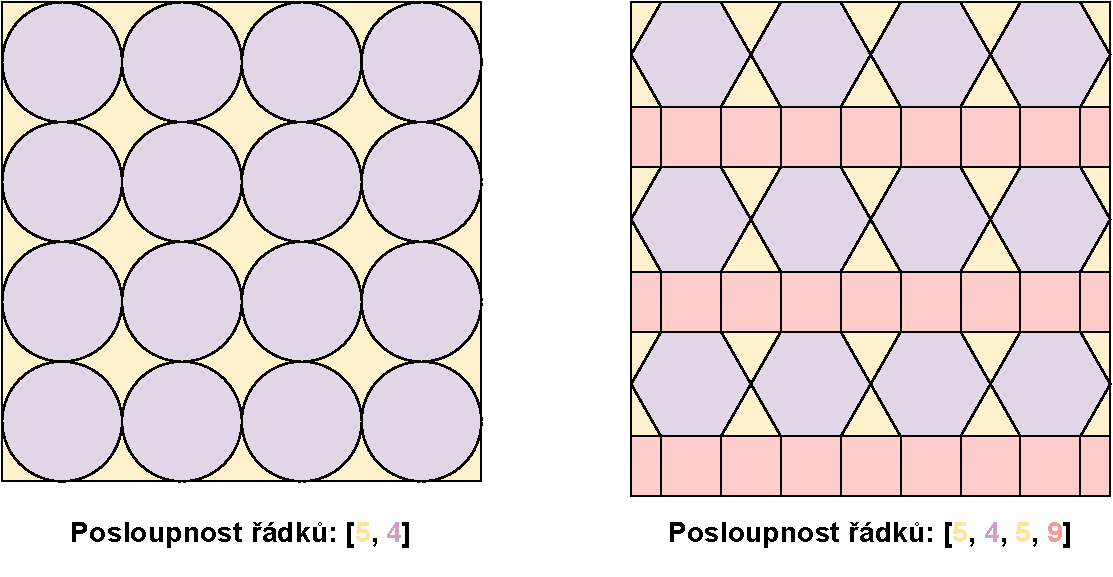
\includegraphics[width=0.9\textwidth]{obrazky-figures/SekvenceRadku.pdf}
    \caption{Rozložení dlaždic v mřížce a jim přiřazený vzor délek řádků}
    \label{fig:SekvenceRadku}
\end{figure}

Takto načtené dlaždice jsou na řádcích zpravidla ve špatném pořadí, což je způsobeno tím, že je jako první rozpoznána dlaždice s nejvýše položeným pixelem, přičemž dlaždice na jednom řádku často nemají jejich nejvyšší bod na stejné horizontální linii. Řádky dlaždic v poli jsou z toho důvodu seřazeny funkcí \verb|sort_tiles()| dle souřadnice \emph{x} jejich prvního nalezeného bodu. 

Uvedený postup však stále zanechává jeden problém -- výstupní pole dlaždic obsahuje řádky různých délek, se kterým není schopný celulární automat pracovat, jelikož očekává na vstupu obdélníkové pole. Aby bylo tvaru obdélníku dosaženo, jsou z obou stran kratších řádku přidány virtuální dlaždice pomocí funkce \verb|to_rect_shape()|, dokud není dosaženo délky nejdelšího řádku.

\subsubsection*{Implementace rozpoznání mřížky}
V této části se budeme zabývat zejména implementací výplně a modifikací mřížky při rozpoznání, které je řízeno automaty definovanými v sekci \ref{section:recogTheory}.  Jako první hledá funkce \verb|_find_new_beginning_()| počátek nové dlaždice stavovým řízením automatu A1 (\ref{secA1}). Pokud automat skončí v akceptujícím stavu, vloží na místo čtecí hlavice znak $F_B$ \linebreak (\verb|Alphabet.FILL_BEGIN|). Na tomto místě začíná výplň dlaždice funkcí \verb|_fill_tile_()|. Proces výplně je ilustrován na obrázku \ref{fig:prubehVyplnePOpis} v předchozí kapitole. Nejdřív je spuštěn automat A2 (směrem dolů, \ref{secA2}), a poté A3 (směrem nahoru, \ref{secA3}). Pokud čtecí hlavice těchto automatů narazí na znak $E$ (\verb|Alphabet.EMPTY|), uloží se jeho souřadnice do seznamu \verb|buffer|. Po skončení činnosti A2 a A3 se všechny znaky na mřížce, které jsou uloženy v seznamu, změní na znak $F$ (\verb|Alphabet.FILL|). Poté se spustí funkce \verb|_find_new_fill_beginning_()| z posledního znaku $F_B$, která vloží při akceptujícím stavu nový znak $F_B$. Pokud skončí v~zamítajícím stavu, výplň je ukončena.

Všechny znaky $F$ a $F_B$, přidané při rozpoznání, jsou uloženy do dlaždice \verb|Tile| ve vrstvách v pořadí, ve kterém byla vyplněna. Každá dlaždice má uloženou svoji výplň, a rozpoznání tak vždy probíhá pouze jednou, na začátku. 

\subsection*{Abstrakce a transformace dlaždic}

V modulu \verb|tiles.py| se nachází implementace tříd \verb|Tile| a \verb|TileGrid|, které pojímají vstupní mřížku jako obdélníkové dvou-dimenzionální pole dlaždic tak, aby na něm mohly být prováděny transformace pomocí celulárního automatu definovaného v sekci \ref{section:sortingCA}. Modul obsahuje definice dlaždic včetně funkcí, které je zpracovávají. 

\subsubsection*{Třída Tile}
Dlaždice zapsána formou třídy v jazyku Python má následující strukturu dílčích atributů:
\begin{itemize}
    \item \verb|fill_layers| představuje seznam výplňových vrstev dlaždice, které jsou načteny při rozpoznání. Každá výplňová vrstva je seznamem souřadnic \verb|(row, column)| vstupní mřížky.
    \item \verb|color| je barva dlaždice ve formátu \verb|(red, green, blue)| a v rozsahu 0--255.
    \item \verb|shape| reprezentuje odkaz na objekt třídy \verb|Shape|, který je abstrakcí vnitřního tvaru dlaždice.
    \item \verb|size| je velikost dlaždice definovaná jako součet výplňových vrstev.
\end{itemize}

\subsubsection*{Třída TileGrid}
Pole dlaždic je realizováno v atributu \verb|grid| třídy \verb|TileGrid| jako dvourozměrný seznam. Z~hlediska funkcionality jsou v této třídě implementovány všechny operace nad polem dlaždic od jejich přidání, po konverzi na výstupní obraz. V sekcích níže jsou popsány metody, které tyto operace implementují.

\subsubsection*{Načítání dlaždic}
Zde popsané metody společně zajišťují korektní načtení dlaždic do dvou-dimenzionálního pole.

\begin{itemize}
    \item \verb|add_tile()| na základě čísla načtené dlaždice a sekvence délek řádků přidá dlaždici na konec posledního řádku, nebo na začátek nového řádku tak, aby délky řádků odpovídaly vstupní sekvenci.
    \item \verb|sort_tiles()| seřazuje řádky dlaždic vzestupně dle sloupce z první položky seznamu \verb|fill_layers|. 
    \item \verb|to_rect_shape()| zajišťuje obdélníkový tvar seznamu. Pokud řádky nemají stejnou délku, jsou ke kratším řádkům z obou stran přidány virtuální dlaždice, dokud není dosaženo délky nejdelšího řádku.
\end{itemize}

\subsubsection*{Počáteční permutace}

Po načtení je potřeba dlaždicím přiřadit atributy na základě vybrané barevné palety a~seznamu povolených tvarů. Rozhodl jsem se přiřazení provést náhodně, jelikož smyslem navrženého celulárního automatu je vytvářet uspořádání, jehož průběh bude dobře vidět na náhodně uspořádané počáteční konfiguraci. Výčet atributů a forma jejich náhodného přiřazení je popsaná v následujícím výčtu.

\begin{itemize}
    \item \textbf{Přiřazení barev} se odvozuje od vstupní barevné palety. Položka palety obsahuje barvu a hodnotu představující kumulativní četnost jejího výskytu, což například znamená, že kumulativní četnost výskytu třetí barvy v~seznamu představuje četnost výskytu prvních třech barev.
    Kumulativní četnost je v rozsahu $\langle  0, 1 \rangle$ a je využita pro náhodný výběr pomocí generátoru pseudonáhodných čísel \verb|random.random()|. V~rámci náhodného výběru je sekvenčně procházen seznam barev, a pokud je kumulativní četnost menší než pseudonáhodné číslo, vybereme barvu a ukončíme cyklus. Takto přiřadíme s novým pseudonáhodným číslem barvu každé dlaždici. Barva je přiřazena vnitřnímu tvaru i pozadí s jinými pseudonáhodnými čísly. Uživatel si může vybrat, zda chce používat pro tvary a pozadí odlišné palety, nebo pouze jednu pro oba případy.
    \item \textbf{Přiřazení tvarů} je realizováno jako náhodný výběr z diskrétního rovnoměrného rozložení. Tvary jsou uloženy v seznamu délky $l$, ze kterého vybereme tvar nacházející se na náhodně vygenerovaném indexu $i$ z rovnoměrného diskrétního rozložení o rozsahu $\langle  0, l - 1 \rangle, i \in \mathbb{Z}$.
    \item \textbf{Přiřazení velikosti vnitřního tvaru} je přiřazení pseudonáhodného čísla $s$ vygenerovaného z rozsahu $\langle  \frac{S}{4}, S\rangle, s \in \mathbb{Z}$, kde $S$ představuje velikost dlaždice. Jako spodní hranice velikosti byla vybrána vyšší hodnota než jedna z důvodu nízké estetiky příliš malých tvarů.
\end{itemize}

\subsubsection*{Transformace nad polem dlaždic}

Transformace pole dlaždic spočívá v implementaci celulárního automatu definovaného v~sekci \ref{section:sortingCA}. Funkce \verb|apply_transformation_step()| představuje přechod jednoho stavu celulárního automatu do druhého. Výstupem funkce je nová konfigurace pole dlaždic. Přechod je realizován aplikací tranzitivní funkce na všechny dlaždice v poli. Tranzitivní funkce se neprovede, pokud vybraná sousední buňka přesahuje hranice pole. Převod relativního směru množiny $D$ z definice celulárního automatu na absolutní souřadnice pole dlaždic je realizováno funkcí \verb|_direction_to_coords_()|. Uspořádání na základě barev je implementováno jako porovnání součtu RGB hodnot. Vyšší hodnota součtu značí světlejší barvu, tmavší barvy reprezentují nižší hodnoty.

\subsubsection*{Konverze do výstupního obrázku}

Barevný obraz na výstupu je generován pomocí pole dlaždic, ve kterém se nachází informace o tom co nakreslit, jakou barvou, a jakým způsobem. Kromě pole dlaždic je při konverzi využito i vstupní mřížky, která slouží k inicializaci rozměrů výstupního obrázku, a slouží jako reference při kreslení vnitřních tvarů a případném odstranění hranic $B$. Konverze je implementována ve funkci \verb|to_image()|.

Jako první je inicializováno výstupní pole barvou hranic, kterou zadá uživatel. Poté se provede iterace přes výplňové vrstvy všech dlaždic, a na výstupní pole se barevně vykreslí jejich pozadí. V případě, že je vnitřní tvar konturou dlaždice, dojde pouze ke změně barvy pozadí na barvu vnitřního tvaru tam, kde kontura začíná. V opačném případě se vyplní celá dlaždice barvou pozadí, a vnitřní tvar je poté vykreslen funkcí \verb|draw()|. 


\subsection*{Vnitřní tvary}

Vnitřní tvary dlaždic se nachází v třídě \verb|Shape| modulu \verb|shapes.py|. Vnitřní tvar dlaždic se skládá z typu, velikosti, a barvy.
Součástí tohoto modulu je implementace vykreslení vnitřních tvarů do výstupního obrazu, a inicializace šablon vnitřních tvarů pomocí celulárního automatu definovaného v sekci \ref{section:GrowingCA}.

\subsubsection*{Šablony tvarů}

Šablony tvarů jsou uloženy v seznamu vrstev podobně jako výplň dlaždic s tím rozdílem, že jsou seřazeny od vnitřní vrstvy po vnější, v opačném pořadí vrstev dlaždic. Šablony představují největší možné tvary, které se mohou do dlaždic vejít. Při kreslení tvaru do výstupního obrázku se vždy využije stejný či menší počet vrstev, který dává šablona k~dispozici. Uložení vrstev do paměti ušetří výpočetní čas tím, že není třeba vykreslovat vnitřní tvar pomocí celulárního automatu u každé dlaždice, ale pouze jednou, před začátkem kresby výstupního obrázku. Činnost celulárního automatu, který je modelem pro tvorbu šablon vnitřních tvarů, je blíže popsána v sekci \ref{section:GrowingCA}. 

Dvou-dimenzionální pole, na kterém jsou šablony vytvářeny, je nejprve naplněno souřadnicemi tak, aby se bod $(0, 0)$ nacházel ve středu pole. Inicializace souřadnic pole je znázorněna v tabulce \ref{tab:PoleSablony}, přičemž zlomky, které se v ní vyskytují, jsou zaokrouhleny k~nejbližšímu celému číslu a notace zaokrouhlení je v tabulce pro přehlednost vynechána. 
Souřadnice jsou relativní ke středu vytvářené šablony. V počáteční konfiguraci je v poli vyplněna pouze středová buňka, ve které jsou uloženy souřadnice $(0, 0)$. Výplň, kterou v~dalším stavu automat provede, je uložena do mezipaměti, a poté uložena do šablony jako další vrstva. Výplň končí, pokud je čas současné konfigurace roven velikosti největší dlaždice.

\begin{table}[H]
    \centering
    \begin{tabular}{ c c c c c }
    $\overset{[0,0]}{(-\frac{m}{2},-\frac{n}{2})}$ & $\overset{[0,1]}{(-\frac{m}{2},-\frac{n}{2} + 1)}$ & $\hdots$ & $\overset{[0, n - 2]}{(-\frac{m}{2},\frac{n}{2} - 2)}$ & $\overset{[0, n - 1]}{(-\frac{m}{2},\frac{n}{2} - 1)}$ \\ 
    $\overset{[1 ,0]}{(-\frac{m}{2} + 1,-\frac{n}{2})}$ & $\ddots$ & $\vdots$ & $\reflectbox{$\ddots$}$ & $\overset{[1, n - 1]}{(-\frac{m}{2} + 1,\frac{n}{2} - 1)}$ \\ 
    $\vdots$ & $\hdots$ & $\overset{[\frac{m}{2},\frac{n}{2}]}{(0,0)}$ & $\hdots$ & $\vdots$ \\ 
    $\overset{[m - 2,0]}{(\frac{m}{2} - 2, -\frac{n}{2})}$ & $\reflectbox{$\ddots$}$ & $\vdots$ & $\ddots$ & $\overset{[m - 2,n - 1]}{(\frac{m}{2} - 2,\frac{n}{2} - 1)}$ \\ 
    $\overset{[m - 1,0]}{(\frac{m}{2} - 1, -\frac{n}{2})}$ & $\overset{[m - 1,1]}{(\frac{m}{2} - 1, -\frac{n}{2} + 1)}$ & $\hdots$ & $\overset{[m - 1,n - 2]}{(\frac{m}{2} - 1,\frac{n}{2} - 2)}$ & $\overset{[m - 1,n - 1]}{(\frac{m}{2} - 1,\frac{n}{2} - 1)}$ \\ 
    \end{tabular}
    
    \caption{Relativní souřadnice využité při tvorbě šablony tvaru. V hranatých závorkách jsou indexy pole o rozměrech $m \times n$, v kulatých závorkách jsou relativní souřadnice (zlomky jsou zaokrouhleny na nejbližší celé číslo).}
    \label{tab:PoleSablony}
\end{table}

Šablony jsou do výstupního obrázku přeneseny funkcí \verb|draw()|. Na vstupu funkce je počáteční bod vykreslování, který je zároveň posledním bodem v atributu \verb|fill_layers| dlaždice. Tvar roste z počátečního bodu do prostoru po vrstvách, které jsou uloženy v~šabloně. Počáteční bod je ke každému bodu šablony přičten a výsledkem je absolutní souřadnice bodu ve~výstupním obrazu. Kreslení tvaru končí, pokud bylo dosaženo počtu vrstev specifikovaných velikostí tvaru v atributu \verb|size|.

\subsection*{Barevná paleta}

Barvy pozadí dlaždic a jejich vnitřních tvarů jsou přiřazovány z barevné palety, která je extrahována z libovolného vstupního obrazu. K extrakci barev je využita knihovna \verb|extcolors| \cite{extcolors}, která vytvoří shluky barev na základě vstupního obrazu, a uloží je do seznamu společně s~četností výskytu. V modulu \verb|palette.py| se nachází funkce \verb|img_to_palette()|, která obsahuje implementaci extrakce barevné palety z obrázku. Výstupní paleta se od palety vrácené knihovnou \verb|extcolors| liší ve vyjádření četností výskytu. Navržená funkce četnosti vrácené knihovnou normalizuje z rozsahu $\langle 0, n \rangle$, kde $n$ značí počet všech pixelů vstupního obrázku, do rozsahu $\langle 0, 1 \rangle$. Aby bylo možné z tohoto seznamu vybírat pomocí pseudonáhodně generovaných čísel, transformují se četnosti výskytu na kumulativní hodnoty. Znamená to, že četnost barvy na indexu $i$ seznamu, představuje četnost této barvy, a všech předchozích zároveň.  

\subsection*{Video výstup}

Implementace konverze obrázku na video se nachází v modulu \verb|videoenc.py|. Vstup představuje seznam obrazů, vygenerovaných funkcí \verb|to_image()|, který je předán funkci \linebreak \verb|VideoWriter| z knihovny \verb|cv2| \cite{cv2}. Uživatel může parametrem \verb|scale_factor| specifikovat, zda chce rozlišení výstupního videa zvětšit či zmenšit, v opačném případě si video zachovává stejné rozlišení jako vstupní mřížka. Při konverzi je využito formátu \verb|mp4|, přičemž výstupní video má obnovovací frekvenci jednoho snímku za vteřinu.

\chapter{Testování aplikace a ukázky výstupů} 
\label{testing}

Program, který reprezentuje praktickou část této práce, na výstupu vrací sady obrazů, které společně tvoří video. Vzhledem k tomu, že jsou výstupy aplikace potenciálně hodnotné převážně pro jejich estetický aspekt a pro jejich schopnost kreativně vizualizovat činnost navržených automatů, je není vhodné testovat primárně pomocí formálních metrik. Tato kapitola je koncipována jako názorná ukázka výstupů aplikace. Jejím cílem je předvést možné výstupy v situacích, kdy aplikaci poskytneme validní mřížku, kterou jsme definovali v sekci \ref{section:recogTheory}, a taktéž znázornit chování aplikace v případech, kdy se na vstupu nachází mřížka s vadami. Výstupy stručně zhodnotíme, a popíšeme nastavení programu, při kterém vznikly. 

Testování proběhlo na operačním systému Windows 10 s nástroji, uvedenými v sekci \ref{impl:utils}. Jednotlivé výstupy jsou zároveň dostupné ke shlédnutí na odkazu, který se nachází poznámce pod čarou.\footnote{Video demonstrace výstupů aplikace: \\ \url{https://youtube.com/playlist?list=PLmqY7KSySjDDjWEJPChE_rpowOe25cOXV}}

\section{Vstupní mřížka s artefakty}

Dlaždice vstupní mřížky mohou obsahovat různé vady: jejich hranice mohou být přerušené, nebo se naopak uvnitř dlaždic mohou nacházet hraniční body, které hranice nereprezentují. Tyto chyby mohou být zapříčiněny jak uživatelem, tak modulem, který převádí vstupní obraz na černobílou mřížku. Příklad konverze obrazu na vadnou mřížku se nachází na obrázku \ref{fig:KonverzeSpatneMrizky} níže.

\begin{figure}[H]
    \centering
    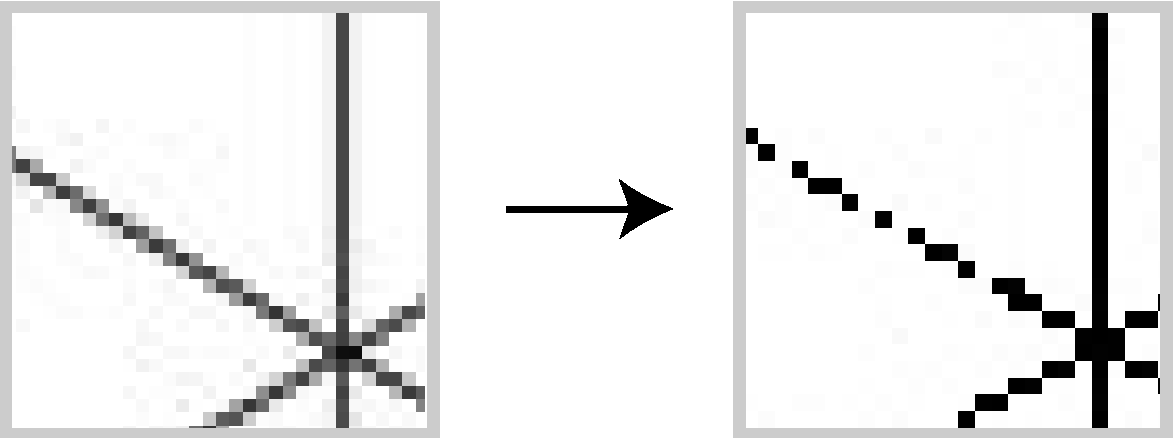
\includegraphics[width=0.7\textwidth]{obrazky-figures/KonverzeSpatneMrizky.pdf}
    \caption{Konverze obrazu špatného rozlišení na mřížku (threshold = 150)}
    \label{fig:KonverzeSpatneMrizky}
\end{figure}

Program vstupní mřížku buď zamítne, nebo se ji pokusí vyplnit s tím, že dlaždice budou na výstupu vypadat více či méně odlišně. K zamítnutí dojde pouze v situaci, kdy procházení směrem dolů přejde za levou hranici obrazu, nebo procházení směrem nahoru přejde za hranice obrazu zprava. Stavové řízení jinými slovy překročí hranice opačné strany, kterou neopisuje, protože není schopné najít jinou cestu. Jelikož v této situaci nelze s výplní pokračovat, ukončí se chybou. Na obrázku \ref{fig:triangles} níže jsou na levé straně znázorněny výsledky výplně s prahovou hodnotou těsně nad hranicí, kde je mřížka zamítnuta.  Na výstupu si můžeme všimnout horizontálních přerušení trojúhelníkových dlaždic, které vznikly v oblastech, kde byly hranice děravé. Můžeme říct, že model rozpoznání má tendenci špatně specifikované dlaždice rozdělovat do horizontálních sekcí, pokud je schopen je přijmout pomocí automatů A2 a A3. Na pravé straně se nachází výstup s vyšší prahovou hodnotou, ve~kterém se artefakty nenachází.

\begin{figure}[H]
    \centering
    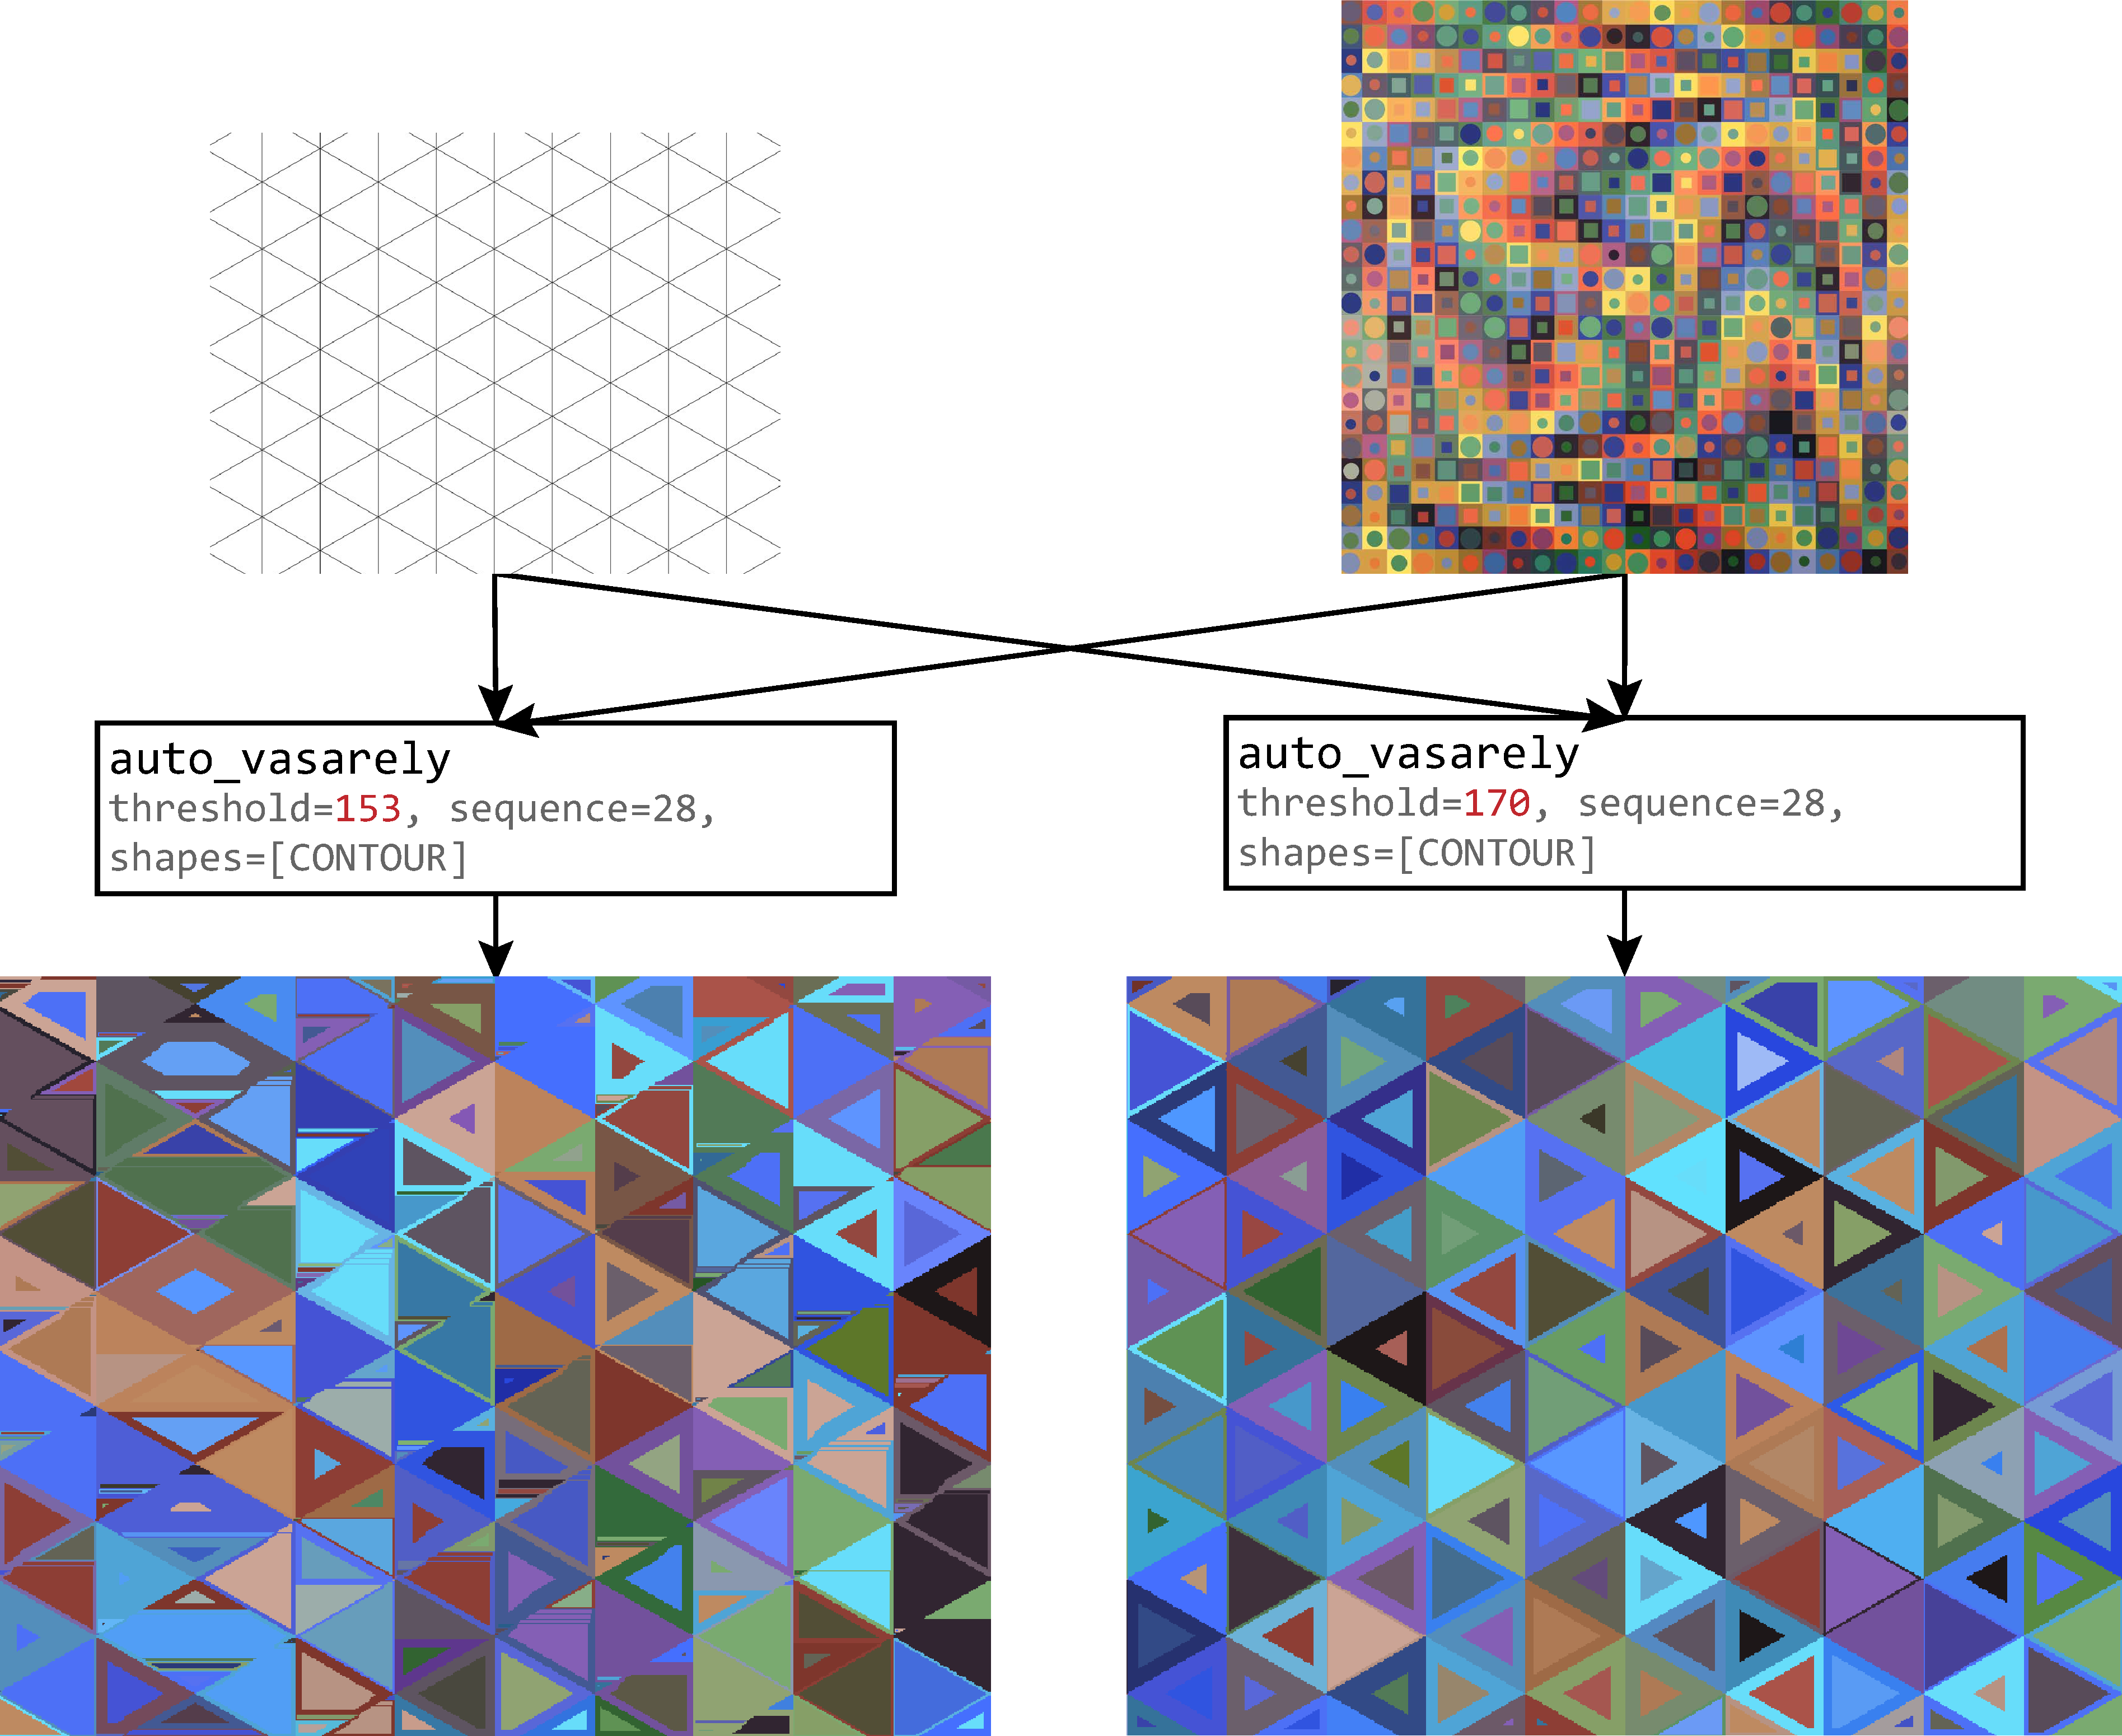
\includegraphics[width=\textwidth]{obrazky-figures/triangles.pdf}
    \caption{Vliv prahové hodnoty na výstup. Na vstupu se nachází trojúhelníková mřížka, barevnou referenci reprezentuje obraz Majus Victora Vasarelyho \cite{majus}. }
    \label{fig:triangles}
\end{figure}

\section{Dobře specifikovaná vstupní mřížka}

V této sekci se nachází čtyři ukázky výstupů, které byly vygenerovány z dobře specifikované mřížky odpovídající kritériím ze sekce \ref{section:recogTheory}. Každý z výstupních obrazů je vygenerován z jiné mřížky, a je vybarven unikátní barevnou paletou. K obarvení je ve všech případech použito jiné už existující umělecké dílo. Převažují díla moderních uměleckých směrů, v rámci kterých umělci studovali barvy v novém kontextu osvobozeném o dosavadní vjemy a inspirace, a~snažili se nacházet nové formy jejich použití. Dalo by se říct, že program akorát mění konfigurace, které moderní umělci našli v jednoduchých geometrických tvarech, a hraje si s~různými uspořádáními jejich barev na dlaždicovém prostoru s novými obrazci. Jeden vstupní obraz -- post-impresionistická krajina Tahiti -- nebyl vybrán z avantgardního uměleckého směru. Z post-impresionistické interpretace momentu v tropické krajině program vytvoří abstraktní mozaiku přímořských barev. U posledního výstupu se naopak ukáže, že vybraný barevný obraz nebyl vhodným kandidátem pro extrakci barev.

\subsection*{Zachování hranic vstupní mřížky}

Ve výstupu, ilustrovaném na obrázku \ref{fig:tilted_squares}, nejsou hranice dlaždic vymazány, ale obarveny barvou středového čtverce obrazu Cosca II \cite{cosca2}, jehož autorem je Victor Vasarely. Původní konfigurace je barevně i tvarově náhodná, s dalšími kroky se však vnitřní tvary a barvy třídí. V třicáté konfiguraci můžeme pozorovat opačný gradient barev pozadí a vnitřních tvarů. Kosočtverce jsou posunuty doleva a čtverce doprava. Na místech, kde se potkává tmavý vnitřní tvar se světlým pozadím můžeme pozorovat souvislost s Vasarelyho barevnou paletou. Nakloněné čtverce pozadí působí dojmem, že se naklání celý obraz. Optická iluze Vasarelyho je tak nahrazena iluzí mřížky, na kterou byly jeho barvy přeneseny.

\begin{figure}[H]
    \centering
    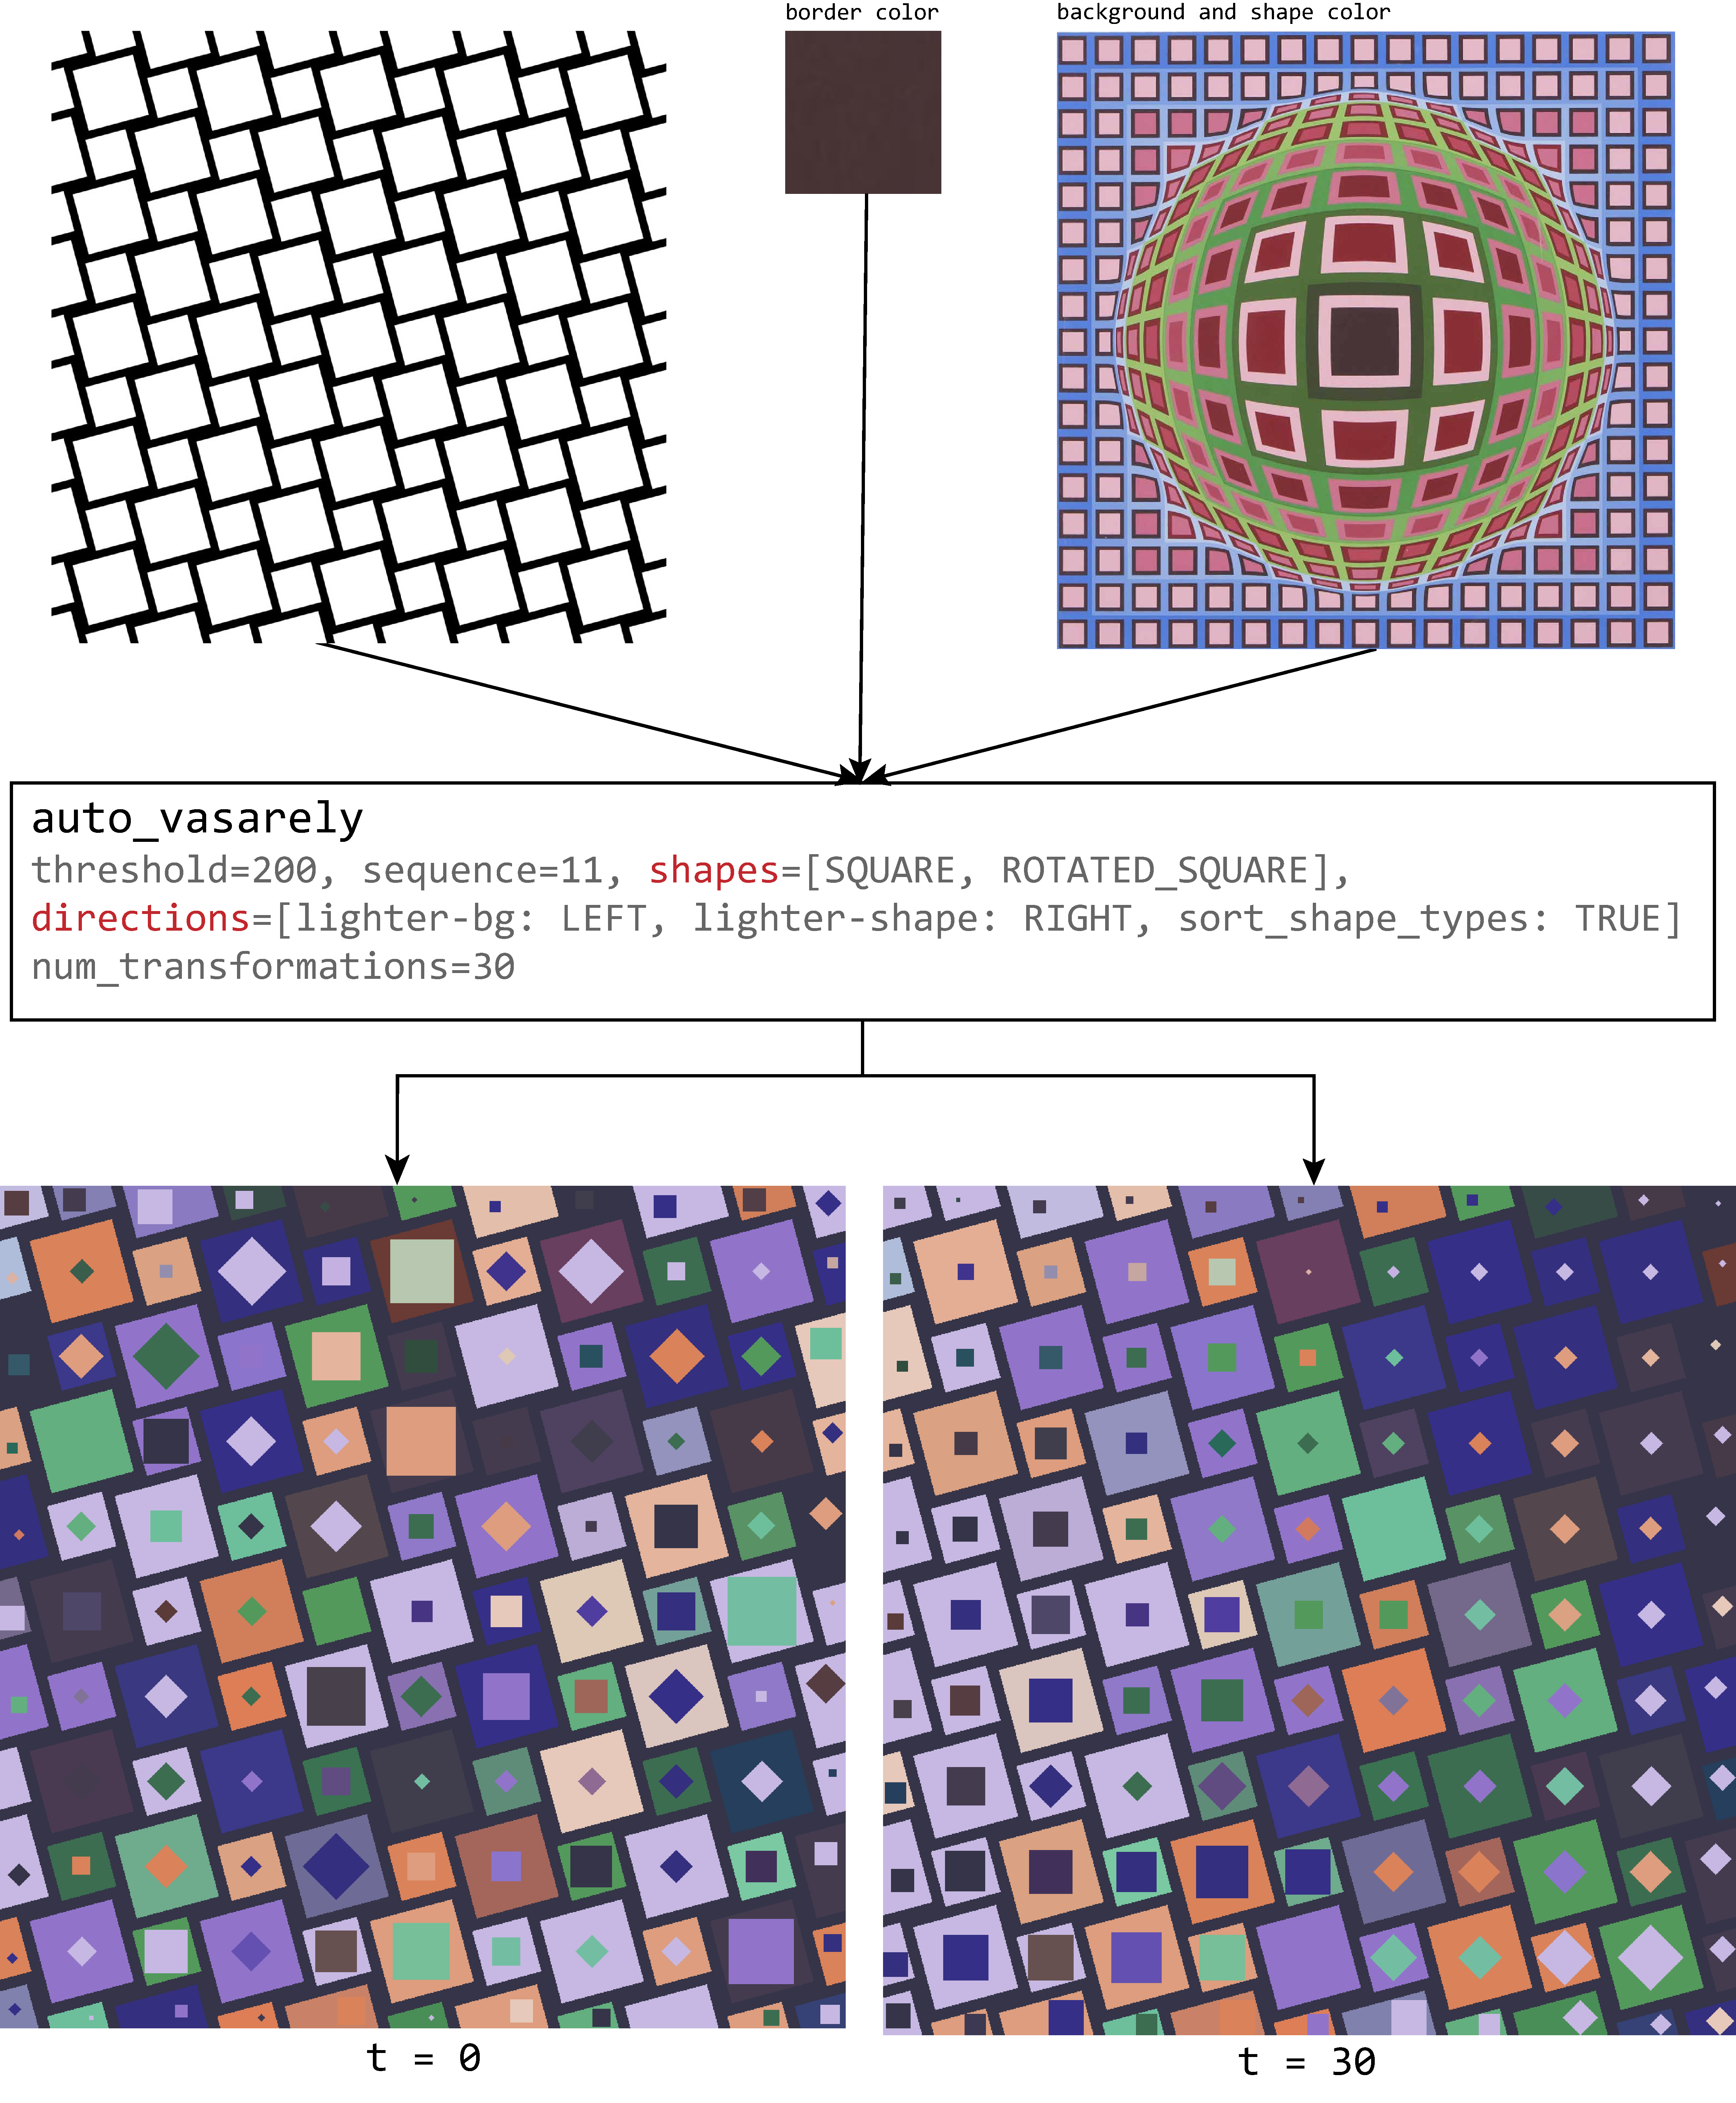
\includegraphics[width=\textwidth]{obrazky-figures/tilted_squares.pdf}
    \caption{Zachování hranic u mřížky s nakloněnými čtverci. Barevná paleta je extrahována z obrazu Cosca II Victora Vasarelyho. Hranice jsou obarveny odstínem středového čtverce Vasarelyho obrazu. \cite{cosca2}. }
    \label{fig:tilted_squares}
\end{figure}

\subsection*{Použití všech vnitřních tvarů a transformací}

Výstupní obrazy v této sekci, znázorněny diagramem \ref{fig:hexagons}, tvoří mozaiku \linebreak z post-impresionistického obrazu Tahitská krajina od Paula Gauguina  \cite{tahiti}. Transformace zde s obrazem korespondují, jelikož byly vybrány tak, aby ve třicáté konfiguraci alespoň trochu odpovídaly barevnému rozložení Gaughinova obrazu. Světlé pozadí se posouvalo nahoru a doleva, aby bylo v rohu dosaženo virtuálního zdroje světla. Uprostřed se míchají různé barvy a odstíny, a dole můžeme na rozdíl od původního obrazu vidět tmavou bažinu. Výstupy v tomto případě obsahují všechny tvary, které jsou s časem tříděny. 

\begin{figure}[H]
    \centering
    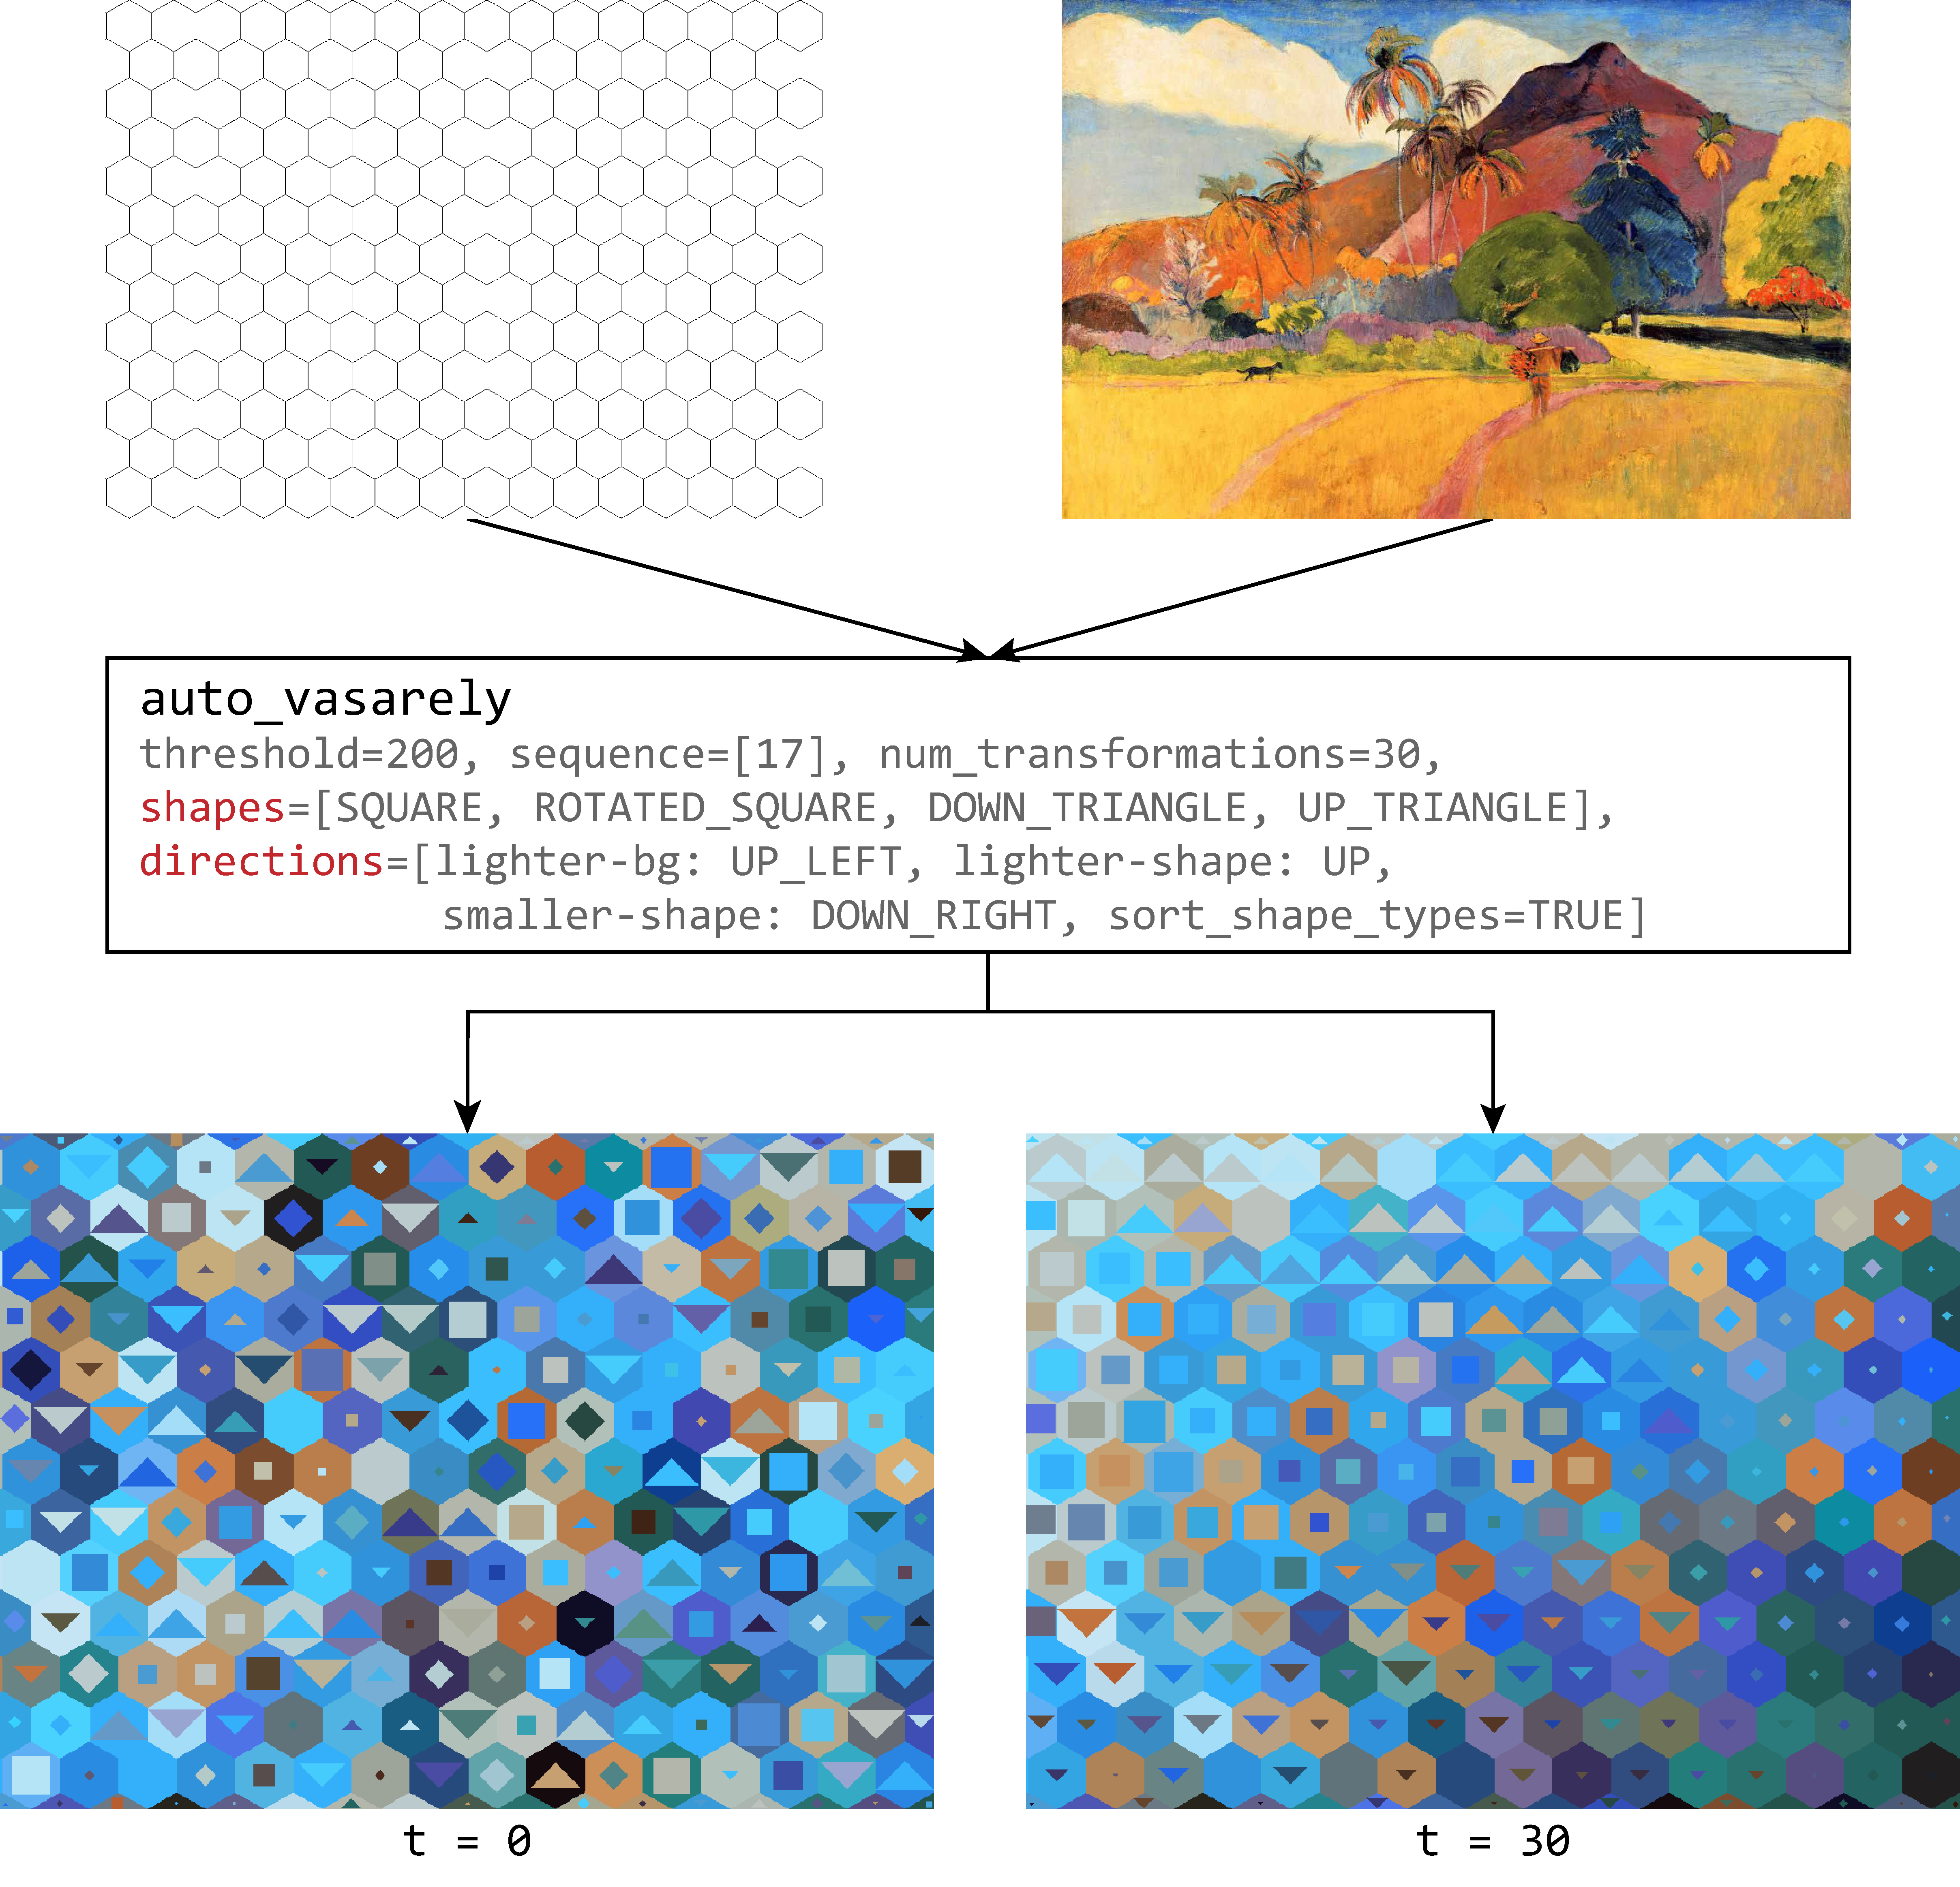
\includegraphics[width=\textwidth]{obrazky-figures/hexagons.pdf}
    \caption{Využití všech vnitřních tvarů a transformací na šestiúhelníkovém poli. Obarvení proběhlo na základě obrazu Tahitská krajína od Paula Gaughina \cite{tahiti}. }
    \label{fig:hexagons}
\end{figure}

\subsection*{Plastický efekt mřížky}

Vstupní mřížka je v této sekci složena z krychlí v dvou-dimenzionální projekci a sama o~sobě vytváří uniformní iluzi hloubky. Jako barevná paleta do mřížky vstupuje suprematistický obraz Kazimira Maleviče \cite{suprematism} s jasně rozlišenými barvami, které jsou naneseny na jednoduché geometrické objekty. V první konfiguraci narušuje spojení mřížky a palety jednu perspektivu, z jaké jsme mohli vnímat původní mřížku. Stejné barvy jsou umístěny na jiné stěny krychle a rozbíjí tak přirozené stínování. Některé krychle se jeví jako vystupující z~obrazu, a některé prostupují dovnitř. V třicáté konfiguraci se trojrozměrný dojem v horní části obrazu úplně rozbíjí díky splývajícím barvám pozadí, a dole přetrvává jen velmi lehce. Vstupy a výstupy jsou znázorněny na obrázku \ref{fig:cubes}.

\begin{figure}[H]
    \centering
    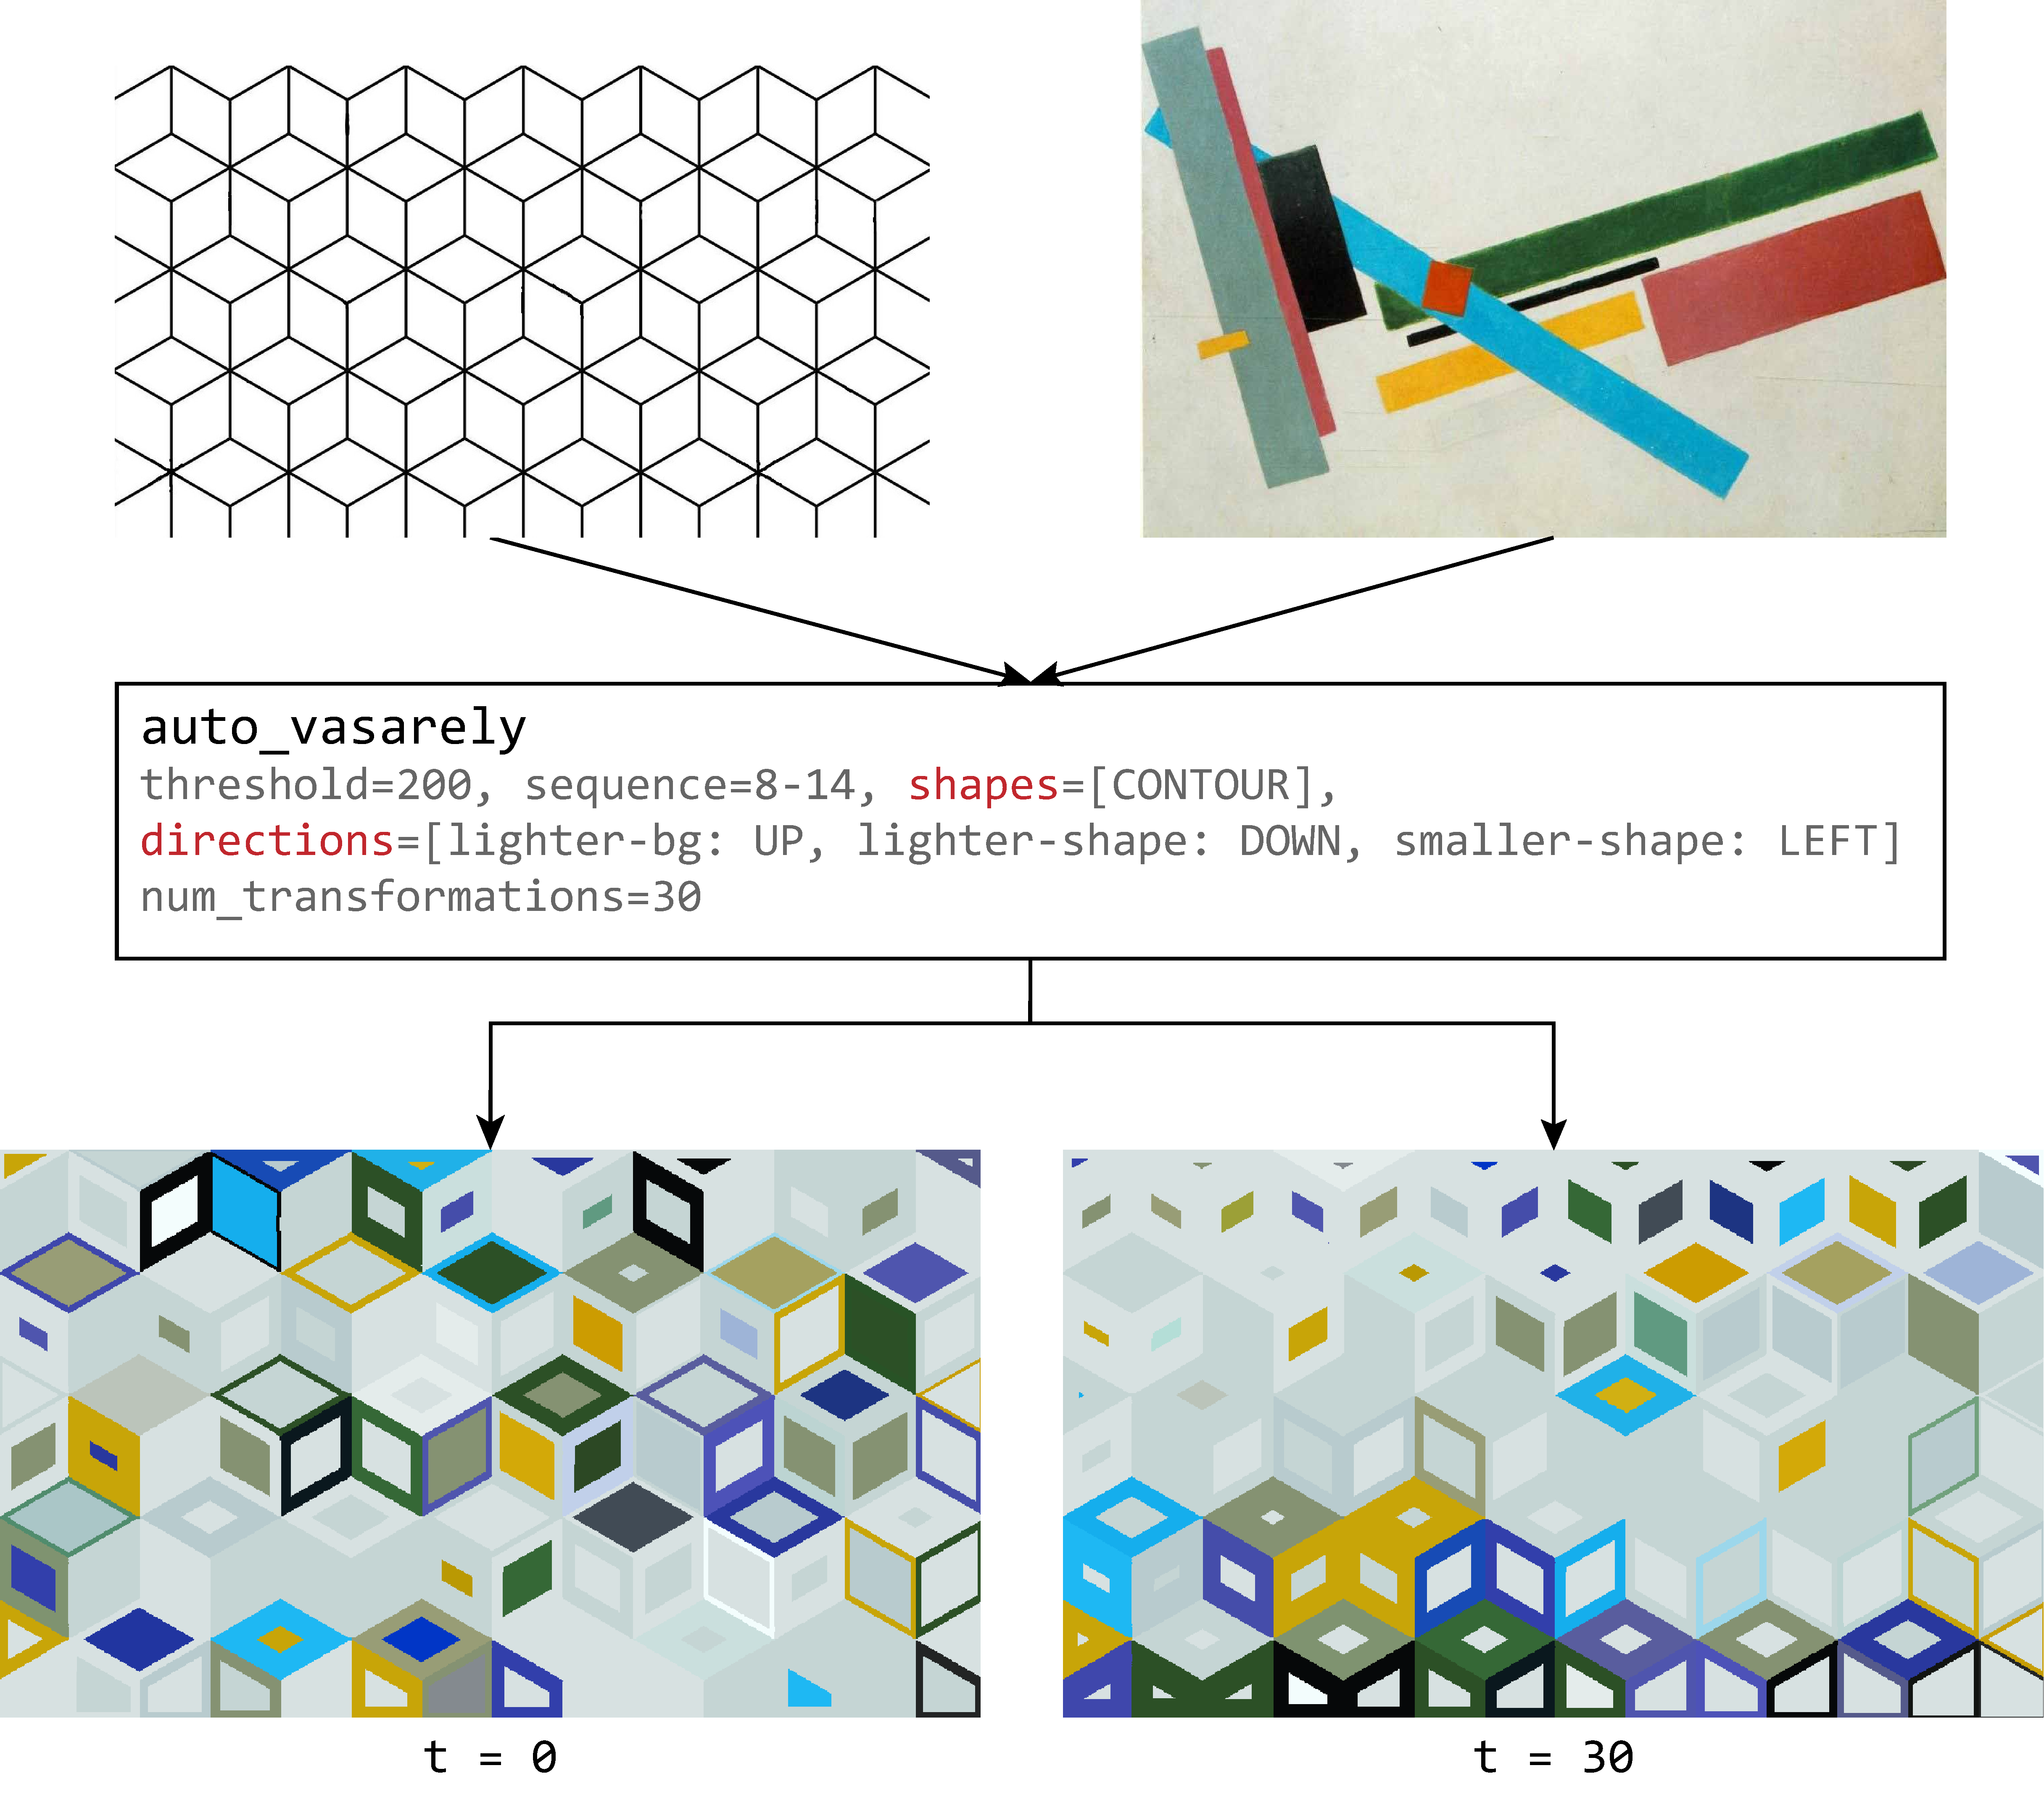
\includegraphics[width=\textwidth]{obrazky-figures/cubes.pdf}
    \caption{Plastický efekt na mřížce s dlaždicemi ve tvaru krychlí obarvené paletou suprematistického obrazu Kazimira Maleviče \cite{suprematism}. }
    \label{fig:cubes}
\end{figure}

\subsection*{Chybně extrahovaná paleta}

Poslední ukázka výstupu, kterou lze vidět na diagramu \ref{fig:square_tiles}, se dle mého názoru nezdařila. Jako mřížka byla použita plocha rozdělená na čtverce o čtyřech sekcích s malými čtverci uprostřed. Paleta byla extrahována z abstraktního obrazu Vasilije Kandinského \cite{yellow}, který obsahuje barevné plochy na žlutém pozadí. Ve výstupním obrazu se však skoro žádná žlutá nenachází, dominuje mu naopak ostře tyrkysová barva, která se v abstraktním díle Kandinského skoro nevyskytuje. Přičinou špatné extrakce by mohl být fakt, že při přiblížení figuruje ve zdánlivě jednolitém žlutém pozadí několik odstínů, které se značně odlišují. Je možné, že došlo zrovna k takové kombinaci odstínů, které byly rozmístěny do shluků k~jiným barvám, než ke žluté. Výstup zároveň ilustruje úskalí v podobě zubatých hran, které plynou z nízkého rozlišení vstupní mřížky. Tento příklad ukazuje, že je někdy potřeba, aby uživatel pro dosažení kýženého výsledku vytvořil z obrazu paletu manuálně, a až následně ji dal aplikaci k extrakci.
\begin{figure}[H]
    \centering
    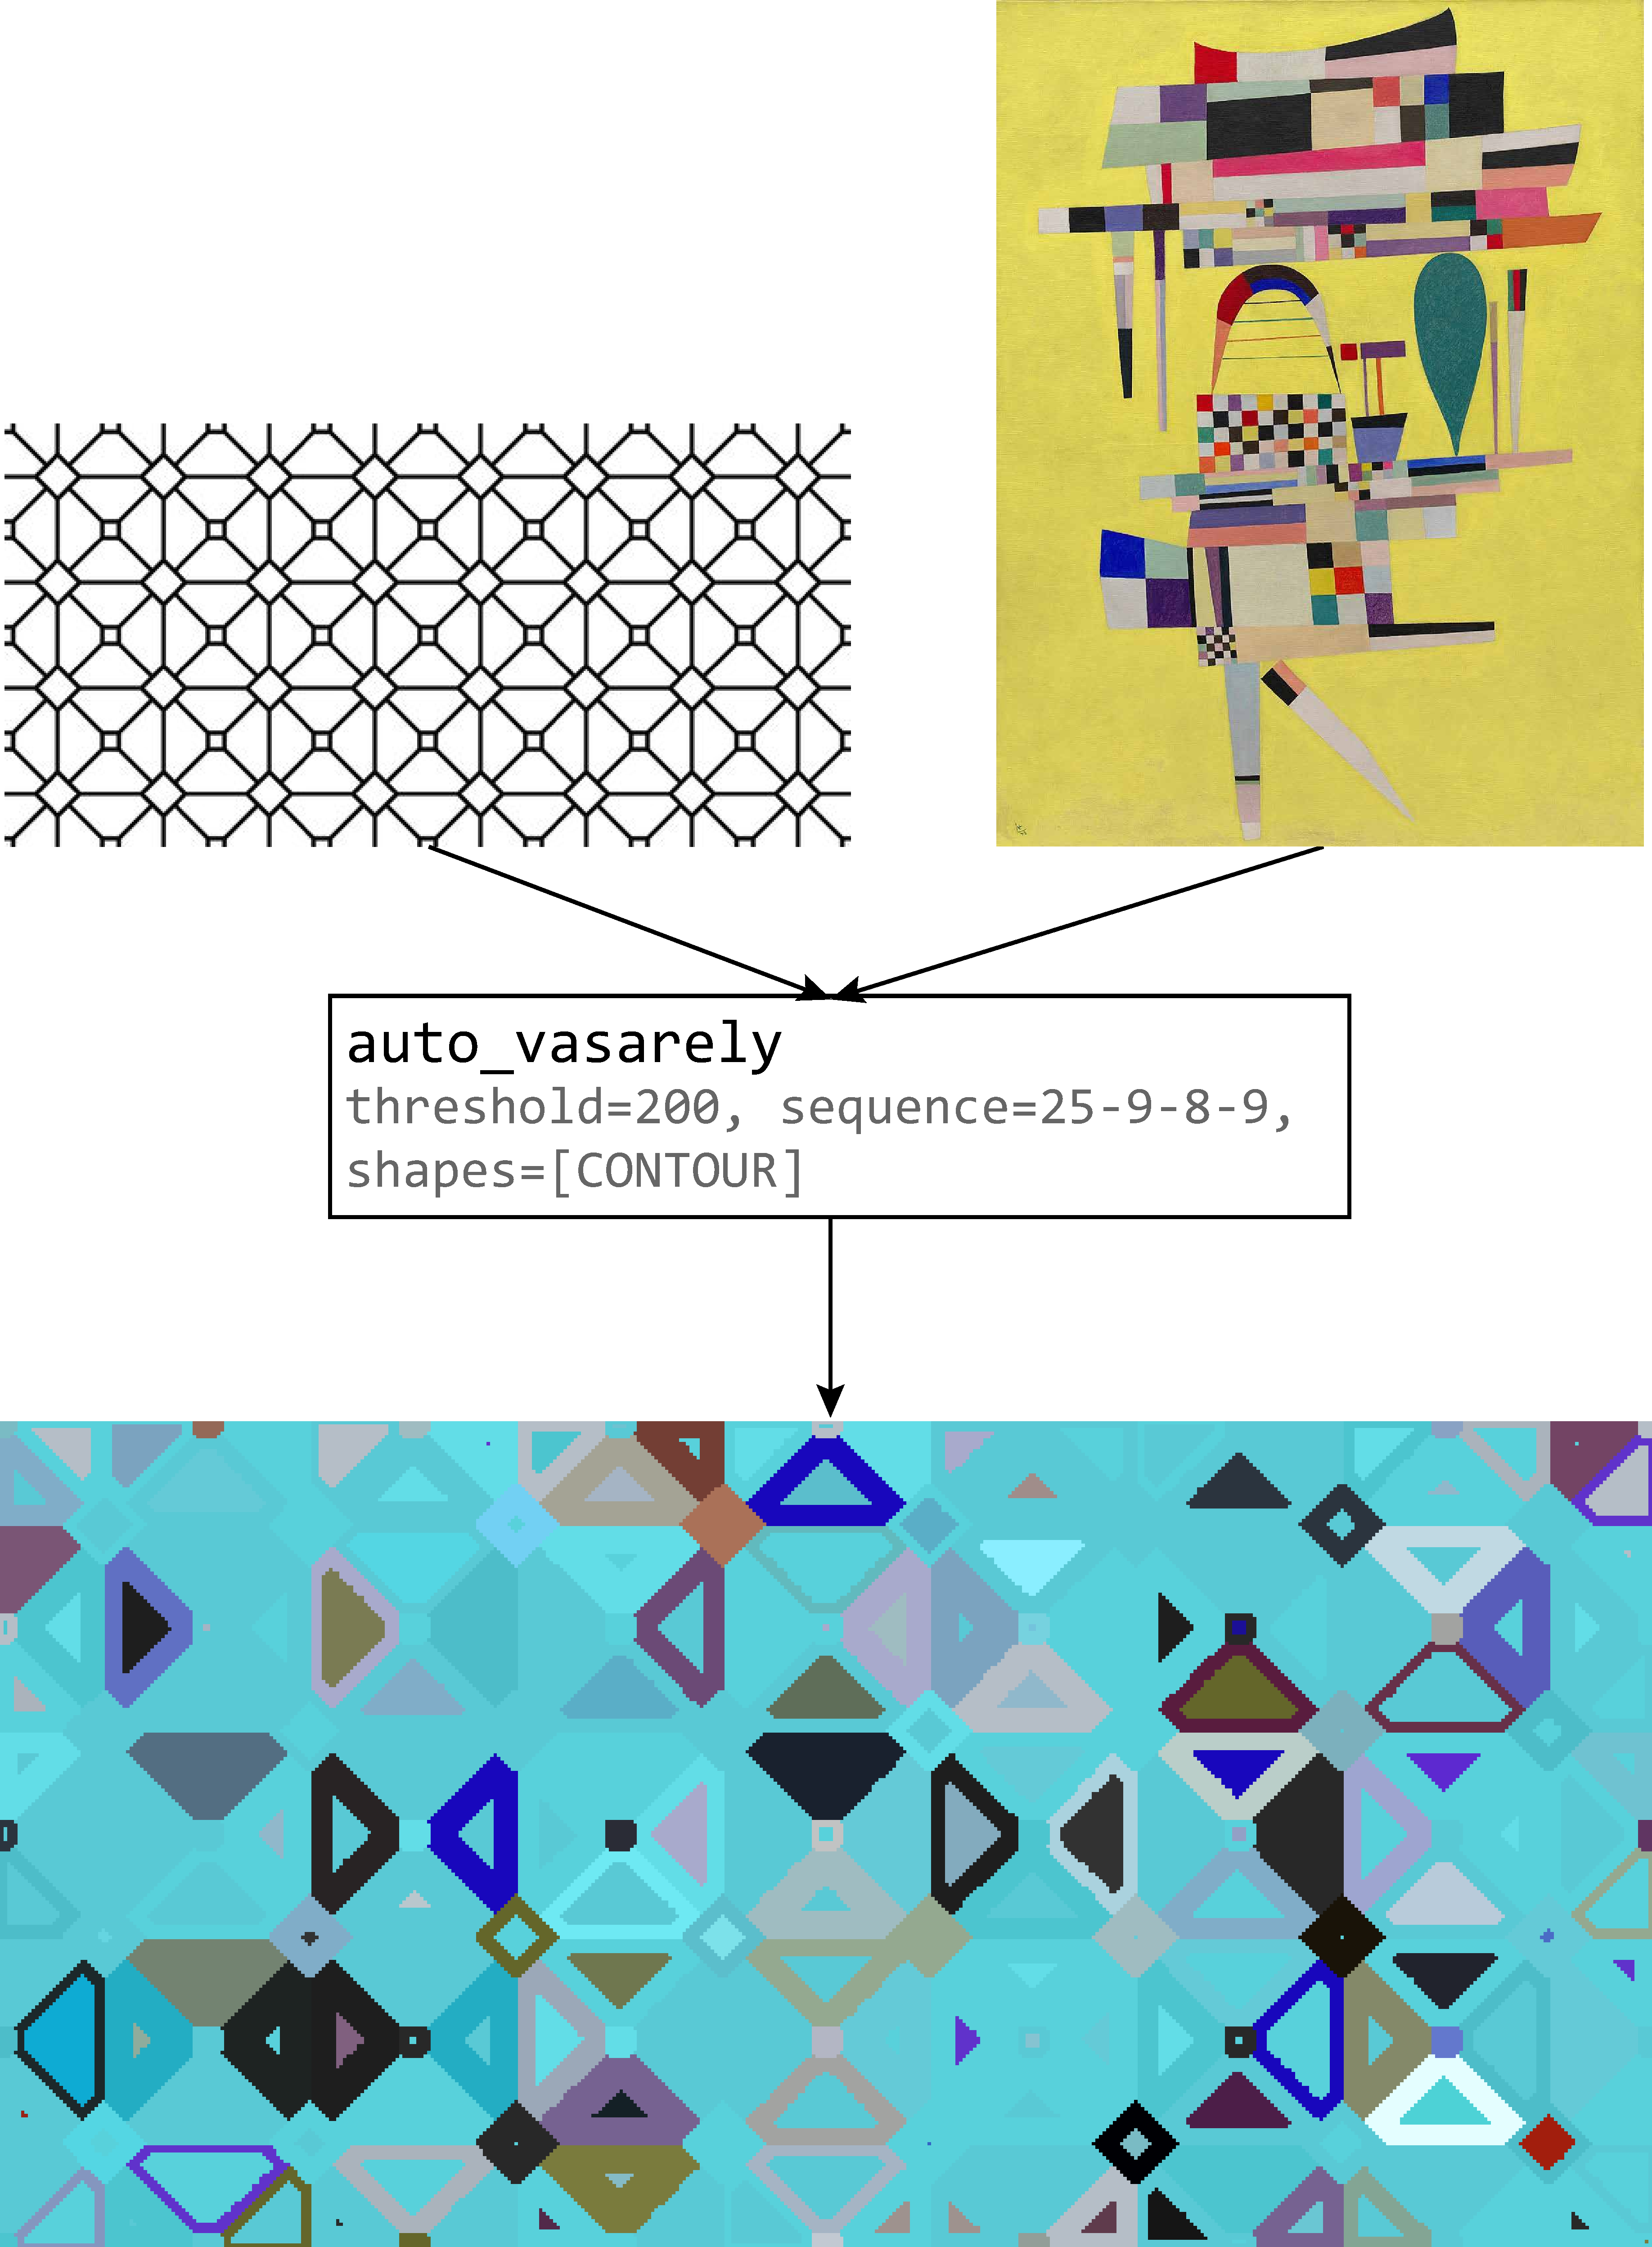
\includegraphics[width=0.8\textwidth]{obrazky-figures/square_tiles.pdf}
    \caption{Ukázka chybně extrahované palety z obrazu Vasilije Kandinského \cite{yellow}. Malé rozlišení vstupní mřížky tvoří na výstupním obrazu zubaté hrany. }
    \label{fig:square_tiles}
\end{figure}

\chapter{Závěr}
\label{conclusion}

Cílem této práce bylo navrhnout a implementovat aplikaci, která vytvoří z barevné reference a mřížky výstupní video, jež ilustruje proces třídění vyplněných dlaždic. Specifikem zde bylo použití formálních modelů, v našem případě celulárních a čtyřcestných dvou-dimenzionálních automatů, s účelem formalizovat řízení rozpoznání, výplně, a transformace vstupní mřížky. 

Návrhu aplikace předcházelo studium již zavedených formálních modelů, a jejich využití při zpracování obrazu. Konkrétně byly pro tuto aplikaci vybrány dva druhy dvou-dimenzionálních automatů: čtyřcestné a celulární. V rámci čtyřcestných automatů jsem studoval modely, které byly využity pro rozpoznání číslic a dopravních značek. V případě celulárních automatů jsem se zaměřil na modely aplikované v umění, konkrétně na jejich využití v textových kompozicích a v tvorbě abstraktních obrazů.

Jako model rozpoznání byly navrženy čtyři čtyřcestné automaty, které řídily proces, jehož výstupem byla abstrakce vstupní mřížky. Dále byl navržen celulární automat, který na základě nastavení tranzitivní funkce třídí dlaždice dle jejich obsahu různými směry. Poslední model, který byl v rámci této práce navržen, představuje celulární automat, který pomocí různých okolí vykresluje čtyři jednoduché tvary. V rámci návrhu byly všechny modely formálně definovány, a čtenáři byly objasněny jejich vlastnosti a princip činnosti.

Tyto modely byly následně implementovány a doplněny o další funkcionalitu tak, aby společně dokázaly vstupní mřížku rozpoznat, vyplnit, a vytvořit v ní několik různých uspořádání. Při implementaci bylo využito několik externích knihoven, které značně ulehčily práci, zejména proces extrakce barev. 

V umělecké dimenzi práce došlo k jistému odklonu od návrhu. S vedoucím práce jsme se dohodli na tom, že se po umělecké stránce budeme místo kompozic textů zaměřovat na vizuální umění. Důvodem k tomuto odklonu bylo studium tvorby Victora Vasarelyho, jehož vize budoucnosti umění byla velkou inspirací pro tuto práci. Seznámil jsem se také s tvorbou jiných uměleckých směrů, například suprematismu, nebo post-impresionismu, s~cílem studovat, které obrazy lze vhodně extrahovat do barevné palety.

Na závěr byl program otestován na několika vstupních mřížkách a barevných referencích. V rámci této části byly zahrnuty jak uspokojivé a estetické výsledky, tak výstupní obrazy, které nesplňovaly očekávané kritéria, nebo obsahovaly artefakty.

Výstup aplikace představuje vizualizaci činnosti třídícího celulárního automatu. Program je schopen uspokojivé extrakce barev z původního obrazu tak, aby zachoval zjevnou spojitost mezi referenčním a výstupním obrazem. Efekt třídění je na dobře vybrané paletě barev viditelný, a mění celkový dojem z vyplněné mřížky první konfigurace například rozbitím její zdánlivé plasticity, nebo vytvořením barevného gradientu, který je podobný rozložení barev v obrazu, z něhož byla extrahována paleta. Rozpoznání mřížky od sebe správně odděluje dobře specifikované dlaždice, a zvolený návrh přidává možnost vybarvit dlaždici po vrstvách směrem ke středu jinými barvami -- můžeme tak dlaždici přiřadit vnitřní objekt stejného tvaru jen pomocí modulu rozpoznání. 

Na několika místech této práce lze identifikovat body, které by bylo vhodné změnit nebo vylepšit. Specifické omezení tvarů dlaždic, které je program schopen rozpoznat, znemožňuje korektní rozpoznání dlaždic s více než jedním maximem a minimem na vertikální ose (např. dlaždice ve tvaru pentagonální hvězdice). V další verzi by se tento nedostatek dal vylepšit úpravou automatů A2 a A3 tak, aby větší počet vertikálních extrémů dlaždic zohlednily. Jiný problém můžeme spatřit v extrakci barev. U některých obrazů neodpovídají extrahované palety původní barevnosti, v jiných případech se palety extrahují lépe, ale výsledné barvy nejsou dostatečně kontrastně odlišeny, nebo tvoří nevhodné párování. Řešení by mohlo představovat výběr jiné knihovny pro extrakci barev, nebo hlubší studium již využité knihovny za účelem nalezení lepšího nastavení parametrů extrakce. Prostor pro zlepšení se dále nachází v primitivním celulárním automatu, který kreslí vnitřní tvary dlaždic. Vhodné rozšíření by mohla představovat komplexnější pravidla v tranzitivních funkcích, která by dovolila automatu kreslit ornamenty nebo krystaly. Aplikace by díky této úpravě mohla tvořit stylově širší množinu výstupů. Transformační efekty by se dalo rozšířit o kolize mezi vnitřními objekty, které by se mohly nacházet pouze na některých místech. Kolize by vznikaly náhodným pohybem vnitřních objektů po dlaždicích v mřížce. Kdyby se dva objekty potkaly, došlo by k jejich zániku, nebo k tvorbě dvou rozdílných objektů.

Program by zároveň šlo doplnit o zcela novou funkcionalitu, například navázáním na jiné období tvorby Victora Vasarelyho přidáním transformací perspektivy. Obraz by se tak mohl sklápět do obrazovky, nebo naopak vyklápět ven. Jiné transformace by naopak mohly mít podobu vlny, která by prostupovala obrazem zleva doprava, a opticky jej zvětšovala obdobně jako lupa, kterou posunujeme nad papírem. Jako poslední uvedu příklad v podobě postupné deformace obrazu v jednom bodě, a dosažení efektu vyboulení nebo díry prostupující dovnitř obrazu.

Využití praktické části práce vidím v podobě dynamického vizuálního pozadí. Konkrétně by výstup aplikace mohl najít uplatnění jako vizuální doplněk koncertů, v rámci světelných show formou promítnutí na fasády domů, nebo jako doplněk současných divadelních performancí. Jako statické dekorativní vzory by naopak mohly být použity jednotlivé snímky videa, ze kterých by si uživatel vybral moment v transformaci obrazu, který se mu nejvíce líbí.

%===============================================================================

% Pro kompilaci po částech (viz projekt.tex) nutno odkomentovat
%\end{document}
